\documentclass[10pt,dvipdfmx]{article}
\setlength{\oddsidemargin}{-1.3truecm}
\setlength{\evensidemargin}{-1.3truecm}
\setlength{\textwidth}{18.5truecm}
\setlength{\headsep}{1truecm}
\setlength{\topmargin}{-2truecm}
\setlength{\textheight}{24truecm}

\usepackage{amsmath,amssymb}
\usepackage{graphicx}
\usepackage{listings,jlisting}
\usepackage{fancybox}
\usepackage{hyperref}
\usepackage{color}

\newcommand{\resa}[1]{ {\textsl{$\rightarrow$ #1}}}
\newcommand{\res}[1]{ {\textsl{#1}}}

%%%%%%%%%%%%%%%%%%%%%%%%%%%
%%% define some colors for convenience
%%%%%%%%%%%%%%%%%%%%%%%%%%%

\newcommand{\mido}[1]{{\color{green}#1}}
\newcommand{\mura}[1]{{\color{purple}#1}}
\newcommand{\ore}[1]{{\color{orange}#1}}
\newcommand{\ao}[1]{{\color{blue}#1}}
\newcommand{\aka}[1]{{\color{red}#1}}

\lstset{language = C,
numbers = left,
numberstyle = {\tiny \emph},
numbersep = 10pt,
breaklines = true,
breakindent = 40pt,
frame = tlRB,
frameround = ffft,
framesep = 3pt,
rulesep = 1pt,
rulecolor = {\color{black}},
rulesepcolor = {\color{black}},
flexiblecolumns = true,
keepspaces = true,
basicstyle = \ttfamily,
identifierstyle = ,
commentstyle = ,
stringstyle = ,
showstringspaces = false,
tabsize = 4,
escapechar=\@,
}

\newcommand{\ubuntubutton}{Ubuntuボタン}

\renewcommand{\thesection}{クラス\arabic{section}}
\renewcommand{\thesubsection}{問題\arabic{section}-\arabic{subsection}}

\title{Python練習問題}
\author{}
\date{}

\begin{document}
\maketitle

\section{}

%%%%%%%%%%%%%%%%%%%%%%%%%%%%%%%%%%%%%%%%%%%
\subsection{{\scriptsize (関数定義)}}
4つの数 $a, b, c, d$ を受け取り, ベクトル $(a, b)$ と $(c, d)$の内積を計算する
関数, {\tt inner(a, b, c, d)} を書き, 適当な例を使って確かめよ.

\begin{itemize}
\item []
\begin{lstlisting}
def inner(a, b, c, d):
    ...

inner(...)
\end{lstlisting}
\end{itemize}

%%%%%%%%%%%%%%%%%%%%%%%%%%%%%%%%%%%%%%%%%%%
\iffalse
\subsection{{\scriptsize (関数定義, import)}}
$a, b, c$を与えられ, 2次方程式:
\[ ax^2 + bx + c = 0 \]
の解(のひとつ; どちらでもよい)を返す関数
{\tt solve\_q(a, b, c)}を書け. ただし, $a \neq 0$
と, 上記方程式が実数解を持つことは仮定して良い.
$\sqrt{\cdot}$を計算する関数は{\tt math}モジュール内の{\tt sqrt}
関数.

できたら, $a, b, c$を与えられ, {\tt solve\_q(a, b, c)}
の結果$x$に対しもう一度$ax^2 + bx + c$を計算する関数
{\tt check\_q(a, b, c)}を書け. もちろん
{\tt check\_q(a, b, c)}は常に, ほぼ0を返すはずである.
ただし誤差の関係からぴったり0にはならない.

%%%%%%%%%%%%%%%%%%%%%%%%%%%%%%%%%%%%%%%%%%%
\subsection{{\scriptsize (関数定義, import)}}
$a, b, c, p, q$を与えられ, 直線:
\[ ax + by + c = 0 \]
と点$(p, q)$の距離を求める関数
{\tt dist\_lp(a, b, c, p, q)}を書け. 
手計算できる適当な数を入れて確かめよ.

%%%%%%%%%%%%%%%%%%%%%%%%%%%%%%%%%%%%%%%%%%%
\subsection{{\scriptsize (関数定義, import)}}
どこかで見た問題: $e$を自然対数の底とする.
以下を計算する関数$f(x)$, $g(x)$を作れ.
\begin{eqnarray*}
f(x) & = & e - \left(1 + \frac{1}{x}\right)^x, \\
g(x) & = & \left(1 + \frac{1}{x}\right)^{x+\frac{1}{2}} - e. \\
\end{eqnarray*}
$x$に色々な数を入れて,$f(x) > 0$, $g(x) > 0$であることを確かめよ.

{\footnotesize 注: 原題(東大2016前期入試数学第1問)は,$f(x) > 0$, $g(x) > 0$
を証明せよというもの.もちろんコンピュータで色々な数に対して,
$f(x) > 0$, $g(x) > 0$が確かめられたからといって,
「すべての」$x$に対してそうだと証明されたなどと思ってはいけないが,
事実としてのもっともらしさはかくも簡単に確認できるという例として.}
\fi

%%%%%%%%%%%%%%%%%%%%%%%%%%%%%%%%%%%%%%%%%%%
\subsection{{\scriptsize (関数定義, import)}}
\label{subsec:sincos}
関数
\[ f(x) = \frac{x}{\sin x} + \cos x \]
を計算するPythonの関数 {\tt f(x)} を書け.

これを使って $x \rightarrow +0$, $x \rightarrow \pi - 0$
の値を計算(予想)せよ.

$\sin$, $\cos$, $\pi$は{\tt math}モジュールの{\tt sin, cos, pi}
という名前でアクセスできる.

%%%%%%%%%%%%%%%%%%%%%%%%%%%%%%%%%%%%%%%%%%%
\subsection{{\scriptsize (関数定義, import, 数値微分)}}
微分係数の定義:
\[ f'(a) = \lim_{h\rightarrow 0} \frac{f(a + h) - f(a)}{h} \]
に従えば,$h$を0に近い数(例えば0.001)に対して,
\[ f'(a) \approx \frac{f(a + h) - f(a)}{h} \]
が成り立つ.これを利用して具体的な$a$に対する微分係数の近似値が簡単に計算できる.
難しい記号操作をする必要はなく,必要なのは,$f(a)$の値が計算できる事だけである.

これを利用して,$\log x$の,$x = a$における
微分係数の近似値を求める関数{\tt log\_prime(a)}を書き,
自分の知る事実
$(\log x)' \approx 1/x$であることを, いくつかの$a$に対して確かめてみよ.
他の関数についてもやってみよ.

なお,$e^x$や$\log x$の値を計算する関数は,
{\tt math}モジュールに,{\tt exp, log}
という名前で提供されている.

注: 上式で$h$をいくらにすればよいかについてはあまり深く
悩む必要はないが以下に注意して適度な値を選ぶ.
\begin{itemize}
\item $h \rightarrow 0$での極限を知りたいのだから, 一般的には小さい方がよい
\item 一方あまり小さくしすぎると, $a + h$の計算が,
  計算機が固定の桁数しか表せないことよる
  「丸め誤差」を起こしてしまい, 逆に誤差が大きくなってしまう
  (最悪の場合, $a + h = a$になってしまう.
  ためしに, $1 + 10^{-16}$ を計算してみよ).
  したがって無闇に$h$を小さくすればいいというわけではない.
  一般には$a$に比べて$h$が相対的に小さすぎては困る.
\end{itemize}

%%%%%%%%%%%%%%%%%%%%%%%%%%%%%%%%%%%%%%%%%%%
\subsection{{\scriptsize (関数の関数)}}
上記では$\log x$の, $a$における導関数の値を求めたが,
全く同じ計算方法で,
$f(x) = e^x$の導関数だろうが
$f(x) = \sin x$の導関数だろうが, 
計算できる.
しかしプログラム上は,関数が変わるたびに似たようなプログラムを
書かなくてはならない.
それよりも「(任意の)関数$f$(と$a$)を受け取り,
その$f'(a)$を求める」関数を書くことができれば便利である.

実はPythonにおいては関数を,
他の関数に渡したり変数に代入したりできるのでこのようなことが素直に可能である.
例えば以下は,「(任意の)関数$f$と値$a$」を
受け取り,$f(f(a))$を計算する関数である.

\begin{itemize}
\item []
\begin{lstlisting}
def twice(f, a):
    return f(f(a))  
\end{lstlisting}
\end{itemize}

たとえば以下で, $\log \log x$を計算する関数が出来上がる.

\begin{itemize}
\item []
\begin{lstlisting}
def double_exp(x):
    return twice(math.log, x)
\end{lstlisting}
\end{itemize}

以上を参考に,「$f$と$a$を受け取り,$f'(a)$を求める」
関数{\tt grad\_at(f, a)}を書け.

\begin{itemize}
\item []
\begin{lstlisting}
def grad_at(f, a):
    ...
\end{lstlisting}
\end{itemize}

これに,{\tt math.sin}, {\tt math.log}などを渡して,
微分係数を計算してみよ.以下の計算結果は,
微分係数の近似式
\[ \frac{f(a + h) - f(a)}{h} \]
で$h$をいくらにするかによって変わるので,
ピタリ一致しなくても気にする必要はない.

\begin{itemize}
\item []
\begin{lstlisting}
grad_at(math.sin, math.pi/3)
@\resa{0.49995669789693054}@   # @$\approx \cos \pi/3$@ 
\end{lstlisting}
\begin{lstlisting}
grad_at(math.log, 20)
@\resa{0.04999987500031722}@   # @$\approx 1/20$@ 
\end{lstlisting}
\end{itemize}

もちろん自分で定義した関数も渡すことができる.

\begin{itemize}
\item []
\begin{lstlisting}
def p(x):
    return x ** 3 + x ** 2

grad_at(p, 2)
@\resa{16.00070001003928}@  # 3x^2 + 2x | x=2
\end{lstlisting}
\end{itemize}

%%%%%%%%%%%%%%%%%%%%%%%%%%%%%%%%%%%%%%%%%%%
\subsection{{\scriptsize (関数を返す関数)}}
関数を別の関数に渡すことができるだけでなく,
関数を, 関数の実行結果として返すこともできる.
文法的には, 関数定義文の{\tt def}も文の一種であるので,
関数の中に書くことができる, ということに過ぎない.
例えば以下は, $a, b, c$を受け取ると,
\[ f(x) = ax^2 + bx+ c \]
という「関数」$f$を返す関数({\tt make\_quad})である.
\begin{itemize}
\item []
\begin{lstlisting}
def make_quad(a, b, c):
    def f(x):
        return a * x * x + b * x + c
    return f  
\end{lstlisting}
\end{itemize}
これに色々な$a$, $b$, $c$を渡すことで色々な2次関数を,
いくらでも生むことができる.
\begin{itemize}
\item []
\begin{lstlisting}
g = make_quad(1, 2, 3)  
h = make_quad(4, 5, 6)  
\end{lstlisting}
\end{itemize}
そうやってできた関数は普通に{\tt def}で定義した関数と同じように呼び出せる.
\begin{itemize}
\item []
\begin{lstlisting}
g(1)
@\resa{6}@  
\end{lstlisting}
\item []
\begin{lstlisting}
h(1)
@\resa{15}@  
\end{lstlisting}
\end{itemize}

この考え方を用いて, 与えられた関数に対してその導関数を返す関数
{\tt derive(f)}を書け.
\begin{itemize}
\item []
\begin{lstlisting}
def derive(f):
    ...  
\end{lstlisting}
\end{itemize}
それを使って例えば以下のようなことができる.
\begin{itemize}
\item []
\begin{lstlisting}
sin_prime = derive(math.sin)
\end{lstlisting}
\end{itemize}
({\tt sin\_prime(x)} $\approx \cos x$ のはず\ldots)
\begin{itemize}
\item []
\begin{lstlisting}
sin_prime(math.pi/4) - math.cos(math.pi/4)
@\resa{-3.535651724428934e-05}@   # @$-3.53... \times 10^{-5}$@
\end{lstlisting}
\end{itemize}

{\tt derive}は関数を受取りまた関数を返すので,
繰り返し適用することもできる. 例えば,
\begin{itemize}
\item []
\begin{lstlisting}
sin_prime2 = derive(derive(math.sin))
\end{lstlisting}
\end{itemize}
{\tt sin\_prime2($x$)} $\approx -\sin(x)$のはずなので,
\begin{itemize}
\item []
\begin{lstlisting}
sin_prime2(math.pi/5) + math.sin(math.pi/5)
@\resa{-8.088125763472398e-05}@  # @$-8.08... \times 10^{-5}$@
\end{lstlisting}
\end{itemize}

この話がややこしく思えた人はあまり悩まなくて良い.
最終的にある$a$における導関数の値$f'(a)$が得たいだけなら,
{\tt grad\_at($f$, $a$)}として計算するのも,
{\tt f\_prime = derive($f$)}としてから{\tt f\_prime($a$)}
とするのも同じことである. {\tt derive}のように,
「関数を返す関数」を書くことができるのは数学で出てくる計算を
素直に表すことができそうだ, と思ってもらえれば良い.
その一つの例が, {\tt derive}を2度適用するだけで,
2階の導関数が導けるということである.

%%%%%%%%%%%%%%%%%%%%%%%%%%%%%%%%%%%%%%%%%%%
\subsection{{\scriptsize (複素数使えます)}}
Pythonでは複素数も容易に扱える.
\begin{itemize}
\item 虚数単位($i$)は, {\tt 1j}または{\tt 1.0j}などと表記
\item 複素数の実部, 虚部は, 式{\tt .real}, 式{\tt .imag}
\item 複素共役は, 式{\tt .conjugate()}
\item 普通の数と同じように, 四則が行える
\item {\tt cmath}というモジュールをimportすると, 
複素数の演算を行う関数が使える
\end{itemize}

例:
\begin{itemize}
\item []
\begin{lstlisting}
1.0j * 1.0j
@\resa{(-1+0j)}@
z = 3.0 + 4.0j
z.real
@\resa{3.0}@
z.imag
@\resa{4.0}@
z * z.conjugate()
@\resa{(25+0j)}@
abs(z)
@\resa{5.0}@
import cmath
cmath.sqrt(1.0j)
@\resa{(0.7071067811865476+0.7071067811865475j)}@
\end{lstlisting}
\end{itemize}

\paragraph{問題:}
複素平面上の原点を中心とする半径1の円を$C$とする.
点${\rm P}(z)$は$C$上にあり, 点A(1)とは異なるとする.
点Pにおける円$C$の接線に関して, 点Aと対称な点を${\rm Q}(u)$とする.
${\displaystyle w = \frac{1}{1-u}}$とおき, $w$と共役な複素数を
$\overline{w}$で表す.

実数$\theta$が与えられると, 
\[ z = \cos\theta + i \sin\theta \]
に対して,
\[ \frac{| w + \overline{w} - 1|}{|w|} \]
を計算するPython関数{\tt g(theta)}を書け.
いくつかの{\tt theta}に対して{\tt g(theta)}を計算してみよ.

\paragraph{注:} $z$から$u$を計算する部分は多少の数学が必要. 
今の主題ではない(し, すでにやった, 思い出したくない, etc.)ので省略したい
人は,
\[ u = -z^2 + 2z \]
を認めても良い.

\paragraph{真面目にやりたい人向けのヒント:}
点$z$の, $x$軸に関して対称な点は$\overline{z}$であることを利用.
一般の直線に関して対称な点を求めたければ,
うまいことその直線が$x$軸になるように回転・平行移動する.

\iffalse
整数$n$が与えられると, 1の$n$乗根($n$個あるうちの, 
最も偏角が小さいもの)を計算する関数{\tt proot(n)}を書け.

これを用いて例えば, {\tt proot(5)}を5乗すると, 
ほぼ1になっていることを確かめよ.

\begin{itemize}
\item []
\begin{lstlisting}
def proot(n):
    ...

proot(5) ** 5
\end{lstlisting}
\end{itemize}
\fi

\newpage
\section{}

%%%%%%%%%%%%%%%%%%%%%%%%%%%%%%%%%%%%%%%%%%%
\subsection{{\scriptsize (visual pythonの練習)}}
Visual Pythonを用いて, 次の3つの矢印を表示する関数
{\tt axes()}を作れ. 
\begin{itemize}
\item 原点と(1,0,0)を結ぶベクトルを赤で
\item 原点と(0,1,0)を結ぶベクトルを青で
\item 原点と(0,0,1)を結ぶベクトルを黄色で
\end{itemize}

\begin{itemize}
\item []
\begin{lstlisting}
from vpython import *
def axes():
    ...

axes()
\end{lstlisting}
\end{itemize}

\iffalse
\begin{center}
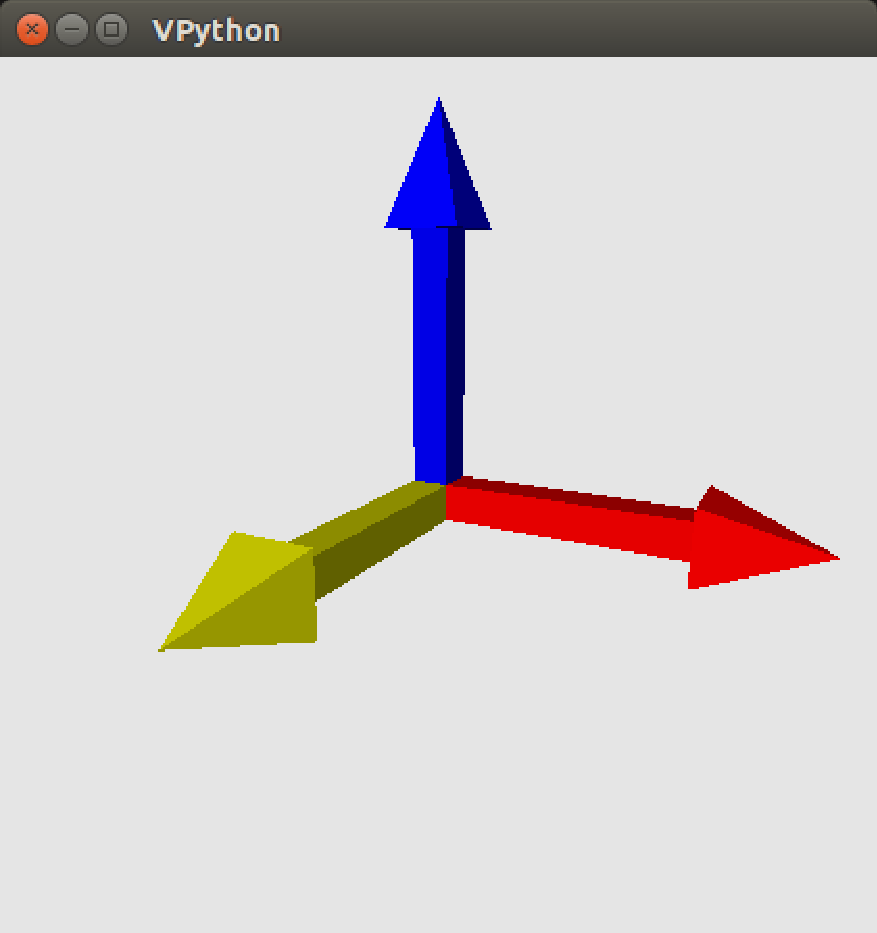
\includegraphics[width=0.25\textwidth]{out/pdf/img/axes.pdf}
\end{center}
\fi

\begin{itemize}
\item 矢印を表示する関数は?
  $\rightarrow$ 授業HPの「有用リンク$\rightarrow$どんなオブジェを作れるか」
  を参照
\item 色を付けるには? 
\begin{lstlisting}
axis(color=color.blue)    
\end{lstlisting}
のようにして色を指定する(上記は青の例). 他のオブジェでも同様.
色に指定できる式は, 上記ページ左のメニューから
``Work with 3D objects'' $\rightarrow$ ``Color/Opacity''
\item 表示窓の操作方法を練習してみよ.
  右クリック$+$ドラッグ, ホイール
\item 見栄えが良くなるよう適宜, 矢印の太さなどを調節してみよ
\end{itemize}

%%%%%%%%%%%%%%%%%%%%%%%%%%%%%%%%%%%%%%%%%%%
\iffalse
\subsection{{\scriptsize (visual pythonで複素平面表示)}}
Visual Pythonは3Dアニメーションが主目的だが, 
$xy$平面だけを用いれば2D表示もできる.
ここではその$xy$平面を複素平面と思って, 
Visual Pythonを複素平面の表示に用いる.

複素数$z$が与えられると, 原点と$z$を結ぶ矢印を表示する関数
{\tt show\_comp(z)}を書け. それを用い, $z$が与えられると,
$1.0$, $z$, $z^2$, $z^3$を表示する関数
{\tt show\_comp3(z)}を書け. 適当な値を$z$に与えて, 
{\tt show\_comp3(z)}を実行してみよ. 

\begin{itemize}
\item 前問同様, 矢印の太さは適宜調節したほうが見栄えがよい
\item わかりやすくなるよう色を調節できればしてみよ
\item 複素数の掛け算は, 
複素平面上でどのような図形的意味に対応していたか思い出して,
結果を眺めてみよ
\end{itemize}
\fi

%%%%%%%%%%%%%%%%%%%%%%%%%%%%%%%%%%%%%%%%%%%
\subsection{{\scriptsize (visual pythonの練習)}}
visual pythonを用いて,「天井」から「バネ」で吊るされた「球」
を表示する関数{\tt mass\_spring()}を作れ.

\begin{itemize}
\item []
\begin{lstlisting}
from vpython import *
def mass_spring():
    ...

mass_spring()
\end{lstlisting}
\end{itemize}

%%%%%%%%%%%%%%%%%%%%%%%%%%%%%%%%%%%%%%%%%%%
\subsection{{\scriptsize (visual pythonの練習)}}
visual pythonを用いて,メタン分子(${\rm CH}_4$)っぽいものを表示する関数
{\tt methane()}を作れ.

\begin{itemize}
\item []
\begin{lstlisting}
from vpython import *
def methane():
    ...

methane()
\end{lstlisting}
\end{itemize}

%%%%%%%%%%%%%%%%%%%%%%%%%%%%%%%%%%%%%%%%%%%
\subsection{{\scriptsize (visual pythonのvector)}}
\label{subsec:vector}
visual pythonでは,3次元ベクトルを簡単に扱える.
{\tt vector($x$, $y$, $z$)}で,$x, y, z$を成分にもつ3次元ベクトルが出来,
あとは通常の演算や,内積,外積が簡単に計算できる.
\begin{itemize}
\item []
\begin{lstlisting}
from vpython import *
u = vector(1,2,3)
u
@\resa{vector(1, 2, 3)}@
v = vector(4,5,6)
u + v
@\resa{vector(5, 7, 9)}@
u - v
@\resa{vector(-3, -3, -3)}@
u.dot(v)
@\resa{32.0}@
u.cross(v)
@\resa{vector(-3, 6, -3)}@
u.x  (またはu[0])
@\resa{1.0}@
u.y  (またはu[1])
@\resa{2.0}@
u.z  (またはu[2])
@\resa{3.0}@
\end{lstlisting}
\end{itemize}

\begin{itemize}
\item 空間内の3点A, B, C (それぞれ{\tt vector}として与えられる)に対し,
三角形ABCの面積を求める関数{\tt area(A, B, C)}を書け.

\item 空間内の2点A, Bに対し,直線ABと$xy$平面($z = 0$)との交点を求める
関数 {\tt intersect\_xy(A, B)}を書け.

\item それらを用い以下の関数$S(a)$を計算する関数を書け.

$a$を$1 < a < 3$をみたす実数とし,
座標空間内の4点${\rm P}_1(1,0,1)$, ${\rm P}_2(1,1,1)$, ${\rm P}_3(1,0,3)$,
${\rm Q}(0,0,a)$を考える.直線${\rm P}_1{\rm Q}$, ${\rm P}_2{\rm Q}$, 
${\rm P}_3{\rm Q}$と
$xy$平面の交点をそれぞれ${\rm R}_1$, ${\rm R}_2$, ${\rm R}_3$として,
三角形${\rm R}_1{\rm R}_2{\rm R}_3$の面積を$S(a)$とする.
\end{itemize}

{\footnotesize 原題(東大2016前期入試数学第3問)は,
この$S(a)$を最小にする$a$とその時の$S(a)$を求めよというもの.
ここではさしあたり$S(2) = 4$となることを確認しておけばよい.}

\newpage
\section{}

%%%%%%%%%%%%%%%%%%%%%%%%%%%%%%%%%%%%%%%%%%%
\subsection{{\scriptsize (繰り返しfor, range)}}\label{sec:newton}
次で定まる数列の第$n$項を計算する関数{\tt a(c, n)}を書け.
\begin{eqnarray}
a_0 & = & c, \\
a_n & = & \frac{1}{3} \left(2a_{n-1} + \frac{c}{a_{n-1}^2}\right) \;\; (n > 0).
\end{eqnarray}

これは$\sqrt[3]{c}$に収束する数列で, 
ある程度大きな$n$に対して, 
{\tt a($c$, $n$)}を計算すればそれが, $\sqrt[3]{c}$の近似値となる.

{\tt a($c$, $n$)}を3乗して, 結果がほぼ$c$と同じになるか確かめよ.

for文を一回繰り返す毎に
$a_n$の値を表示するprint文を挿入して,
$\sqrt[3]{c}$に収束していく様子を表示してみよ
(これは,計算結果が思うようにでない場合の最も基本的な調査手段).

\begin{itemize}
\item []
\begin{lstlisting}
def a(c, n):
    ...  

a(5, 100000) ** 3
\end{lstlisting}
\end{itemize}

\paragraph{参考:} 一般に, $f(x) = 0$の解を求めるのに以下のニュートン法が用いられる.
\begin{eqnarray}
a_0 & = & c, \\
a_n & = & a_{n-1} - f(a_{n-1})/f'(a_{n-1}) \;\; (n > 0).
\end{eqnarray}
これが{\bf 収束するならば}, $x = x - f(x)/f'(x)$を満たす$x$,  
すなわち$f(x) = 0$を満たす$x$に収束することは明らか. 
本問はこれを, $f(x) = x^3 - c$に適用したものである.

ただし, 収束するとは限らないので無条件に使えるわけではない.

計算機で何かを求めるとき, 
このようなに「欲しい答えに収束するような数列」
を使って計算することは非常に多い.


%%%%%%%%%%%%%%%%%%%%%%%%%%%%%%%%%%%%%%%%%%%
\iffalse
\subsection{{\scriptsize (繰り返しfor, range)}}
どこかで見た問題(原作: 東大前期入試2015理系数学 第4問).

数列$\{ p_n \}$を以下のように定める.
\[ p_0 = 1, \quad  p_1 = 2, \quad p_{n+2} = \frac{p_{n+1}^2 + 1}{p_{n}} \; (n \geq 0) \]

\begin{itemize}
\item [(1)] $n$に対して$p_n$を計算するPython関数{\tt p(n)}を書け.
\begin{itemize}
\item []
\begin{lstlisting}
def p(n):
    ...  
\end{lstlisting}
\end{itemize}

\item [(2)] $n$に対して以下の$x_n$
\[ x_n = \frac{p_{n+1}^2 + p_n^2 + 1}{p_{n+1}p_n} \]
を計算するPython関数{\tt x(n)}を書き, {\tt x(0), x(1), x(2), \ldots}
を表示せよ.
\begin{itemize}
\item []
\begin{lstlisting}
def x(n):
    ...  

for i in range(100):
    print x(i)
\end{lstlisting}
\end{itemize}
\end{itemize}

注: 原作は「上記の$x_n$が$n$によらず一定」を証明せよというもの.
\fi

%%%%%%%%%%%%%%%%%%%%%%%%%%%%%%%%%%%%%%%%%%%
\subsection{{\scriptsize for文}}
\begin{itemize}
\item [(1)] 2整数$a$, $b$に対し, 積:
  \[ a \times (a + 1) \times \cdots \times b \]
  を計算する関数{\tt prod(a, b)}を書け
\item [(2)] 以下の数列:
  \[ a_n = \frac{{}_{2n+1}C_{n}}{n!} \]
  が整数になる$n \geq 1$を, 実際に計算して予想せよ.
\end{itemize}

%%%%%%%%%%%%%%%%%%%%%%%%%%%%%%%%%%%%%%%%%%%
\subsection{{\scriptsize (数値積分)}} 
\label{subsec:integrate}
積分の定義式:
\begin{equation}
\int_a^b f(x)\,dx = \lim_{\forall i|x_{i+1}-x_i| \rightarrow 0} \sum_{i=0}^{n-1} f(x_i) (x_{i+1} - x_i)
\end{equation}
に従えば,十分大きな$n$に対して,右辺を計算すればそれが積分の近似値となる:
\begin{equation}
\int_a^b f(x)\,dx \approx \sum_{i=0}^{n-1} f(x_i) (x_{i+1} - x_i).
\label{eq:integ}
\end{equation}
ここで, $a = x_0 < x_1 < \cdots < x_n = b$である.

関数$f$と,積分区間$a$, $b$, 点の数$n$を受け取り,積分:
\[ \int_a^b f(x)\,dx \]
の近似値を, $[a, b]$を$n$等分して式(\ref{eq:integ})の右辺を計算することで求める関数
{\tt integrate(f, a, b, n)}を書け.

書けたらそれを使って好きな積分, 例えば
\[ \int_0^1 \sqrt{1 - x^2}\, dx \]
の近似値を求めよ.

for文内に,足されている$f(x_i)$の値を表示するprint文を挿入してみよ
(計算結果がおもうようにでない場合の最も基本的な調査手段).

\begin{itemize}
\item []
\begin{lstlisting}
def integrate(f, a, b, n):
    ...

def circ(x):
    return math.sqrt(1 - x * x)

integrate(circ, 0.0, 1.0, 1000000)
\end{lstlisting}
\end{itemize}

\paragraph{参考:} この方法は, 計算機で積分を計算する常套手段で, 
手計算の時のように,
原始関数を求めずに実行することができる. 
必要なのは任意の点に対して, $f(x)$
が計算できること{\bf だけ}である.

%%%%%%%%%%%%%%%%%%%%%%%%%%%%%%%%%%%%%%%%%%%
\iffalse
\subsection{{\scriptsize (数値積分)}} 
どこかで見たシリーズ.

関数$h(x)$を次のように定める.
\[ 
h(x) = \left\{
\begin{array}{ll}
-\frac{\pi}{2}\sin(\pi x) & (|x|\leq 1\mbox{のとき}) \\
 0                        & (|x|> 1\mbox{のとき}) \\
\end{array}
\right.
\]

\begin{itemize}
\item [(1)] 上記の関数$h(x)$をPythonの関数として書け
(場合分けにはif文を使うと良い).
\begin{itemize}
\item []
\begin{lstlisting}
def h(x):
    ...  
\end{lstlisting}
\end{itemize}

\item [(2)] そして$I_n$を以下で定める.
\[ I_n = n^2 \int_{-1}^{1} h(nx) \log (1 + e^{x+1}) \, dx \]

$n$が与えられたら$I_n$(の近似値)を計算するPython関数{\tt I(n)}
を書け. それを用いて大きな$n$に対する$I_n$の値を計算してみよ.
\end{itemize}

\begin{description}
\item [原作:] 東大前期入試2015理系数学 第6問.
\item [注1:] 原作は上記の$I_n$の, $n \rightarrow \infty$としたときの
極限値を求めよというもの. 答えは$-e/(1+e)$. 
計算結果がこれに近くなかったら何か間違っている
(Pythonで$e$は{\tt math}モジュールを{\tt import}して, {\tt math.e}).
\item [注2:] $I_n$を計算する際, 区間をどのくらい細かく分割しなくては
ならないか, 検討せよ.
\end{description}
\fi

%%%%%%%%%%%%%%%%%%%%%%%%%%%%%%%%%%%%%%%%%%%
\subsection{{\scriptsize if文}}
どこかで見たシリーズ.

3辺の長さが$a, b, c$である三角形が,
鋭角三角形であるかどうかを判定する関数
(鋭角三角形であれば1, そうでなければ0となる)
{\tt acute\_abc(a,b,c)}を書け.
\begin{itemize}
\item 注1: $a, b, c$の大小は仮定してはいけない.
\item 注2: $(a,b,c) = (5, 2, 2)$のように,
三角形をなさない場合もあるのでその場合も正しく0を返すこと.
\end{itemize}

これを利用して,複素数$z$に対し,複素平面上の3点A(1), B($z$), C($z^2$)
が鋭角三角形をなすかを判定する関数{\tt acute\_z(z)}を書け.

\begin{itemize}
\item []
\begin{lstlisting}
def acute_abc(a, b, c):
    ...  

def acute_z(z):
    ...  
\end{lstlisting}
\end{itemize}

{\footnotesize 注: 原題(東大2016前期入試数学第4問)は,
{\tt acute\_z($z$)}が1となる範囲を図示せよというもの.
後にmatplotlibを使って可視化する.}

%%%%%%%%%%%%%%%%%%%%%%%%%%%%%%%%%%%%%%%%%%%
\iffalse
\subsection{{\scriptsize for $+$ ifの組み合わせ}}
どこかで見たシリーズ.

$n$, $m$に対し, 
\[ 
{}_n\mbox{C}_m \equiv \frac{n!}{m!(n-m)!}
\]
を計算するPython関数{\tt choose(n, m)}を書け. これを用い, 
$m$を2015以下の正の整数としたとき, 
${}_{2015}\mbox{C}_m$が偶数となる最小の$m$を求めよ.

{\footnotesize 注: 原題(東大2015前期入試数学第5問)}

%%%%%%%%%%%%%%%%%%%%%%%%%%%%%%%%%%%%%%%%%%%
\subsection{{\scriptsize for $+$ ifの組み合わせ}}
\ref{subsec:vector}を拡張し,$S(a)$の,$1 < a < 3$
における最小を達成する$a$を求めよ.
すべての$a$に対して$S(a)$を計算することは当然無理なので,
ここでは単純に,1から3を$n = 1000000$等分し,
それらの中の最小値を求める.
\fi


%%%%%%%%%%%%%%%%%%%%%%%%%%%%%%%%%%%%%%%%%%%
\subsection{{\scriptsize 最小値, for $+$ ifの組み合わせ}}
与えられた関数$g$を, 区間$[a, b]$において最小とする$x$を
求めるPython関数 {\tt minimize($g$, $a$, $b$)}を書け.
それを利用して,

\begin{itemize}
\item \ref{subsec:sincos}で定義した関数
{\tt f($x$)}を最小にする
$x$を求めよ.

\item \ref{subsec:vector}で定義した関数{\tt S($a$)}を
最小にする$a$を求めよ.
\end{itemize}

注: $x$を$a$から$b$の間で十分細かく動かして,
その中で$f(x)$が一番小さかったときの$x$を答えれば良い.
どれだけ十分細かくすればよいかのきちんとした判断は難しいし,
どれだけ細かくしても正しく求まらない関数(例: 連続でない関数)もある.
ここではそのへんの厳密さにはこだわらなくて良い.
\begin{itemize}
\item []
\begin{lstlisting}
def minimize(g, a, b):
  ...
\end{lstlisting}
\item []
\begin{lstlisting}
minimize(f, 1e-4, math.pi - 1e-4)  # f : 1-2で定義したもの
@\resa{1.5707963267948963}@
\end{lstlisting}
\item []
\begin{lstlisting}
minimize(S, 1 + 1e-4, 3 - 1e-4)  # S : 2-4で定義したもの
@\resa{2.0}@
\end{lstlisting}
\end{itemize}

%%%%%%%%%%%%%%%%%%%%%%%%%%%%%%%%%%%%%%%%%%%
\subsection{{\scriptsize for $+$ ifの組み合わせ}}
\begin{itemize}
\item [(1)]
  関数$g$と2数$a \leq b$が与えられると,
  方程式$g(x) = 0$が$[a, b]$の範囲で解を持てば
  そのうちの一番小さい解を返し, 持たなければ
  $b$より大きな任意の値を返す関数
  {\tt min\_root(g, a, b)}を書け.

注: 厳密な計算は難しい(一般には不可能). ここでは,
十分小さな$h$に対して, $g(x)$と$g(x+h)$
の符号が異なるかまたはどちらかが0(つまり
$g(x) \cdot g(x+h) \leq 0$)であれば,
$x+h$が解であると考える(もちろんこれは近似解).
区間$[a,b]$内で$x$を少し($h$)ずつ動かして上記を計算していく.

\item [(2)] {\tt min\_root}を用い, 
  \[ x^3 - 3a^2 x = b \]
が解を3つ持ち, かつ3解を$\alpha < \beta < \gamma$としたとき
$\beta > 1$となるかを判定する(真であれば1, 偽であれば0を返す)
関数$p(a, b)$を書け.
\end{itemize}

%%%%%%%%%%%%%%%%%%%%%%%%%%%%%%%%%%%%%%%%%%%
\iffalse
\subsection{{\scriptsize for $+$ ifの組み合わせ}}
\ref{sec:newton}を拡張.
初期値$c$と関数$f$, 許容誤差$\epsilon$が与えられると,数列
\begin{eqnarray}
a_0 & = & c, \\
a_n & = & a_{n-1} - f(a_{n-1})/f'(a_{n-1}) \;\; (n > 0).
\end{eqnarray}
の項を次々と計算し,$|f(a)| < \epsilon$となる$a$が見つかったら
それを返す関数{\tt newton(f, c, eps)}を書け.
ただし,1000000回繰り返して見つからなかったら,
任意の値を返して良い.

零点を持つ適当な多項式を定義し,その根が求まるか試してみよ.

\begin{itemize}
\item []
\begin{lstlisting}
def newton(f, c, eps):
    ...

def poly(x):
    return (x - 2) * (x - 3) * (x - 4)  

newton(poly, 100, 1.0e-10)
\end{lstlisting}
\end{itemize}
\fi

\newpage
\section{}

%%%%%%%%%%%%%%%%%%%%%%%%%%%%%%%%%%%%%%%%%%%
\subsection{{\scriptsize (微分方程式)}}
$f$が$x$の(未知の)関数で,
以下の式(微分方程式)
\begin{eqnarray}
y(a) & = & c, \\
\frac{dy}{dx} & = & \frac{1}{y} \\
\end{eqnarray}
を満たすとする. 
この解が $y = \sqrt{2 (x - a) + c^2}$ 
であることは手計算でもすぐにわかる(変数分離法).

以下はそれを計算機にやらせる方法. 一般に,
\begin{eqnarray}
\frac{dy}{dx} & = & f(x ,y)
\end{eqnarray}
という方程式は,その定義に戻れば,
\begin{eqnarray}
\lim_{h\rightarrow 0} \frac{y(x + h) - y(x)}{h} & = & f(x,y)
\end{eqnarray}
ということ.つまり,$h \ll 1$のとき,
\begin{eqnarray}
y(x + h) & \approx & y(x) + f(x, y) h
\label{eq:ord}
\end{eqnarray}
ということ.言い換えれば,ある$x$における$y$の値($y(x)$)
がわかれば,$y(x + h)$が近似できる.そのために必要なものは右辺の
$f(x, y)$だけである.つまり微分方程式の右辺が計算できればよい.

$y(a)=c$から出発して, 
$y(a + h), y(a + 2h), y(a + 3h), \ldots$
を次々に計算していけば,
任意の$x$における$y(x)$ (の近似値)を計算することができる.

与えられた関数$f$, 実数$a$, $b$, $c$に対し, 
\begin{eqnarray}
y(a) & = & c, \\
\frac{dy}{dx} & = & f(x, y) \\
\end{eqnarray}
を満たす$y$の$x = b$における値$y(b)$の
近似値を計算する関数{\tt ord\_solve(f, a, b, c)}を書け.

それを用いて,最初にあげた微分方程式を解き,
$y(2.5)$, $y(5.0)$などを計算してみよ. 
それを厳密解と比較してみよ. 

\begin{itemize}
\item []
\begin{lstlisting}
def f(x, y):
    return 1.0 / y

ord_solve(f, 1.0, 2.5, 1.0)
ord_solve(f, 1.0, 5.0, 1.0)
\end{lstlisting}
\end{itemize}

なおこの考え方は高階の微分方程式でも容易に適用できる.
$x$が$t$の未知の関数とする.このとき,二階の微分方程式の一般形は
以下の形である.
\begin{eqnarray}
x(a)       & = & c, \\
\dot{x}(a) & = & d, \\
\ddot{x}   & = & f(x, \dot{x}, t)
\end{eqnarray}

これを数値計算で解くには,$x(a)=c, \dot{x}(a)=d$から出発して, 
\begin{eqnarray}
\dot{x}(t + h) & = & \dot{x}(t) + \ddot{x}(t) h, \\
x(t + h)       & = & x(t) + \dot{x}(t) h,
\end{eqnarray}
の二つを使って,$x$と$\dot{x}$を求めていく.

\newpage
\section{}

この節の問題はどれも質点の運動をシミュレートし,
それができたらVisual Pythonで可視化(アニメーション)を
行う.

\paragraph{共通事項:}
\begin{itemize}
\item 
まずは,質点の位置や速度を時々(一定時間や一定繰り返し回ごとに)
{\tt print}で,数字として表示する関数を書け.
明らかな間違いを発見するために重要.

\item それが書けたら{\tt print}する代わりに,
Visual Pythonを使ってアニメーションせよ.

\item アニメーションをする際,
質点だけだと,カメラの自動追従機能によって,
物体が動いているように見えない.質点の近くに適当な静止物体(例えば板)をおいて,
動きがわかるようにすると良い.

\item アニメーションを表示するためには物体が動くたびに
{\tt rate($r$)}という関数を呼ぶ.これを呼ばないと,
画面を更新してくれないので,途中経過が表示されず,
最終的な位置だけが突如表示されることになってしまう.
{\tt rate($r$)}は,画面を更新するとともに,
{\tt rate}が秒間$r$回程度呼ばれるよう,
中で時間調整をする.例えば{\tt rate(30)}は,
$1.0 / 30 = 0.03333\cdots$秒程度の時間調整を行う.
アニメーションが実時間に合わせて進行するようにしたいのであれば,
シミュレーション上$h$だけ時間が経過したら,
{\tt rate($1/h$)}を呼びだせばよい.

\item シミュレーションをやりっぱなしでその結果を鵜呑みにする
わけにはいかない.出した結果があっていそうか,確かめるため,
できることをやってみよ.
アニメーション自体が役にたつが他にも手はある.
\begin{itemize}
\item どうなるはずかがわかりやすい設定でシミュレーションしてみる
\item 成り立つはずの物理法則(保存則)が成り立っているか計算してみる
\end{itemize}
など
\end{itemize}

%%%%%%%%%%%%%%%%%%%%%%%%%%%%%%%%%%%%%%%%%%%
\subsection{{\scriptsize (微分方程式 $+$ 可視化 (1))}}
重力加速度を受けて運動する質点の動きをシミュレーションする関数
{\tt point\_mass($x_0$, $v_0$, $T$)}を書け.
\begin{itemize}
\item $T$はシミュレートする時間(時刻0から$T$まで).
\item $x_0$, $v_0$は初期位置,初速とする.
\end{itemize}


\paragraph{チェック項目と発展課題:}
\begin{itemize}
\item ボールを何度で打ち出したら一番遠くまで飛ぶか,
という答えのよく知られた問題があるが,本当にそうなるか確かめてみよ

\item 空気抵抗(速度に比例して速度の反対向きに加わる力)
を加えて見よ.その場合,一番遠くまで飛ぶ角度はどうなるか?

\item 地面や壁があって衝突によって跳ね返るという状況をアニメーションしてみよ
\end{itemize}

%%%%%%%%%%%%%%%%%%%%%%%%%%%%%%%%%%%%%%%%%%%
\subsection{{\scriptsize (微分方程式 $+$ 可視化 (2))}}
万有引力で引き合って運動する2つの質点の動きを,
シミュレーションする
関数{\tt point\_mass2($m_0$, $x_0$, $v_0$, $m_1$, $x_1$, $v_1$, $T$)}を書け.
\begin{itemize}
\item $T$はシミュレートする時間(時刻0から$T$まで).
\item $m_0$, $x_0$, $v_0$は質点0の質量,初期位置,初速度,
\item $m_1$, $x_1$, $v_1$は質点1のそれらとする.
\end{itemize}

初期状態や質量を変えて以下のような状況をシミュレートしてみよ.
\begin{itemize}
\item 太陽と地球
\item 太陽と彗星
\item 連星
\end{itemize}

%%%%%%%%%%%%%%%%%%%%%%%%%%%%%%%%%%%%%%%%%%%
\subsection{{\scriptsize (微分方程式 $+$ 可視化 (3))}}
バネで吊り下げられた質点の動きをシミュレーションする
関数{\tt spring\_mass($m$, $k$, $y_0$, $T$)}を書け.
\begin{itemize}
\item $T$はシミュレートする時間(時刻0から$T$まで).
\item $m$は質量,$k$はバネ定数.
\item $y_0$は初期位置のy座標とする.
但しバネの自然長の位置を0とする.
\item 初速は0, 天井の位置は適当でよい(見た目以外に影響はないので)
\end{itemize}

\paragraph{チェック項目と発展課題:}
\begin{itemize}
\item バネの周期を正しく計算できているか
\item 空気抵抗を入れて減衰振動にしてみよ
\end{itemize}

\newpage

\section{}
%%%%%%%%%%%%%%%%%%%%%%%%%%%%%%%%%%%%%%%%%%%
\subsection{{\scriptsize (リスト内包表記)}}
リスト内包表記を使って以下の関数を,
なるべく短くきれいに書いてみよう.

\begin{enumerate}
\item $a$, $b$, $n$が与えられ,$[a, b]$を$(n-1)$等分する点を
(端点$a, b$を含み$n$点)リストにしたものを返す関数{\tt linspace($a$, $b$, $n$)}.

\begin{itemize}
\item []
\begin{lstlisting}
linspace(1, 2, 5)
@\resa{[1.0, 1.25, 1.5, 1.75, 2.0]}@
\end{lstlisting}
\end{itemize}

\item $n$が与えられ
\[ 1^3 + 2^3 + \cdots + n^3 \]
を返す関数{\tt sum\_cube($n$)}.
以前はループで以下のように書いたものだが, リスト内包表記を使うと?

\begin{itemize}
\item []
\begin{lstlisting}
def sum_cube(n):
    s = 0
    for i in range(1, n+1):
        s = s + i ** 3
    return s
\end{lstlisting}
\end{itemize}

\paragraph{ヒント:} リスト$L$の要素の和を返す関数は{\tt sum($L$)}

\item 関数$f$と,$a$, $b$が与えられ,積分
\[ \int_a^b f(x)\, dx \]
の近似値を計算する関数.これも以前書いたがリスト内包表記を使うと?

\item 関数$f$と,$a$, $b$が与えられ,
\[ \min_{a\leq x \leq b} \{\; f(x)\; \} \]
を求める関数{\tt minimize($f$, $a$, $b$)}.
\paragraph{ヒント:} リスト$L$の最小値を返す関数は{\tt min($L$)}
\begin{itemize}
\item []
\begin{lstlisting}
def q(x):
    return x * x - 4 * x + 3

minimize(q, a, b)
@\resa{-1.0}@
\end{lstlisting}
\end{itemize}

\item 前問で,$f$を最小にする$x$の値も一緒に返す関数
{\tt minimize\_arg($f$, $a$, $b$)}にするには?
\paragraph{ヒント:} タプルをうまく使う.Pythonでは二つのタプルの大小関係は,
いわゆる「辞書式順序」と定義されている.
\[ (a, b) \leq (c, d) \iff a < c \mbox{ または } a = c \mbox{ かつ } b \leq d \]
また,{\tt min}はタプルのリストに対しても働く.
\begin{itemize}
\item []
\begin{lstlisting}
def q(x):
    return x * x - 4 * x + 3

minimize_arg(q, a, b)
@\resa{(2.0,-1.0)}@
\end{lstlisting}
\end{itemize}

\item 同じ長さのリスト$X$, $Y$を受け取り,
それぞれをベクトルとみなした時の内積を返す関数.
\paragraph{ヒント:} zip

動作例:
\begin{itemize}
\item []
\begin{lstlisting}
dot([1,2,3,4], [4,5,6,7]) 
@\resa{60}@
\end{lstlisting}
\end{itemize}
\end{enumerate}

\newpage

%%%%%%%%%%%%%%%%%%%%%%%%%%%%%%%%%%%%%%%%%%%
\section{}
\subsection{{\scriptsize matplotlib (1変数の関数)}}
以下をmatplotlibを使って描画してみよ
\begin{enumerate}
\item 最もプリミティブな確認. リストだけを使って,
点 $(1,1)$, $(2,4)$, $(3,9)$, $(4,16)$をつないだグラフ
\item $y = \sin(x)$のグラフを$0 \leq x \leq 2\pi$の範囲で
{\small (numpyの機能をかっこよく使って)}.
\item $x^2 + y^2 \leq 1$の範囲にランダムにばらまかれた点
{\small (plotの代わりにscatter)}.
\end{enumerate}

\begin{center}
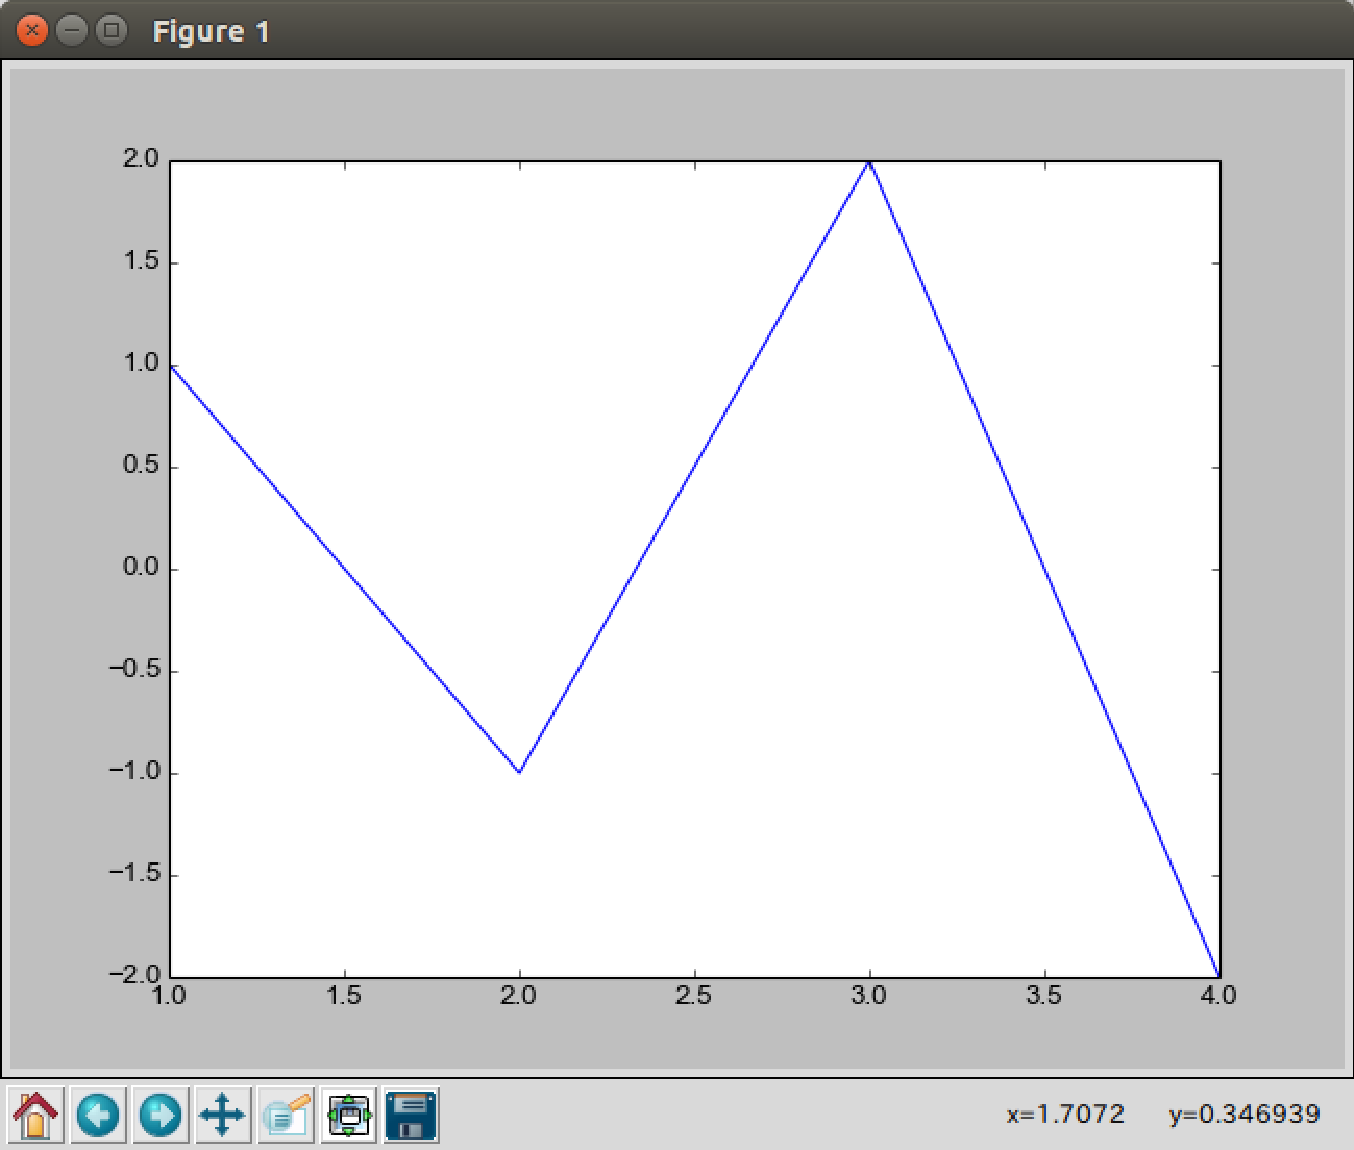
\includegraphics[width=0.3\textwidth]{out/pdf/img/plot_practice.pdf}
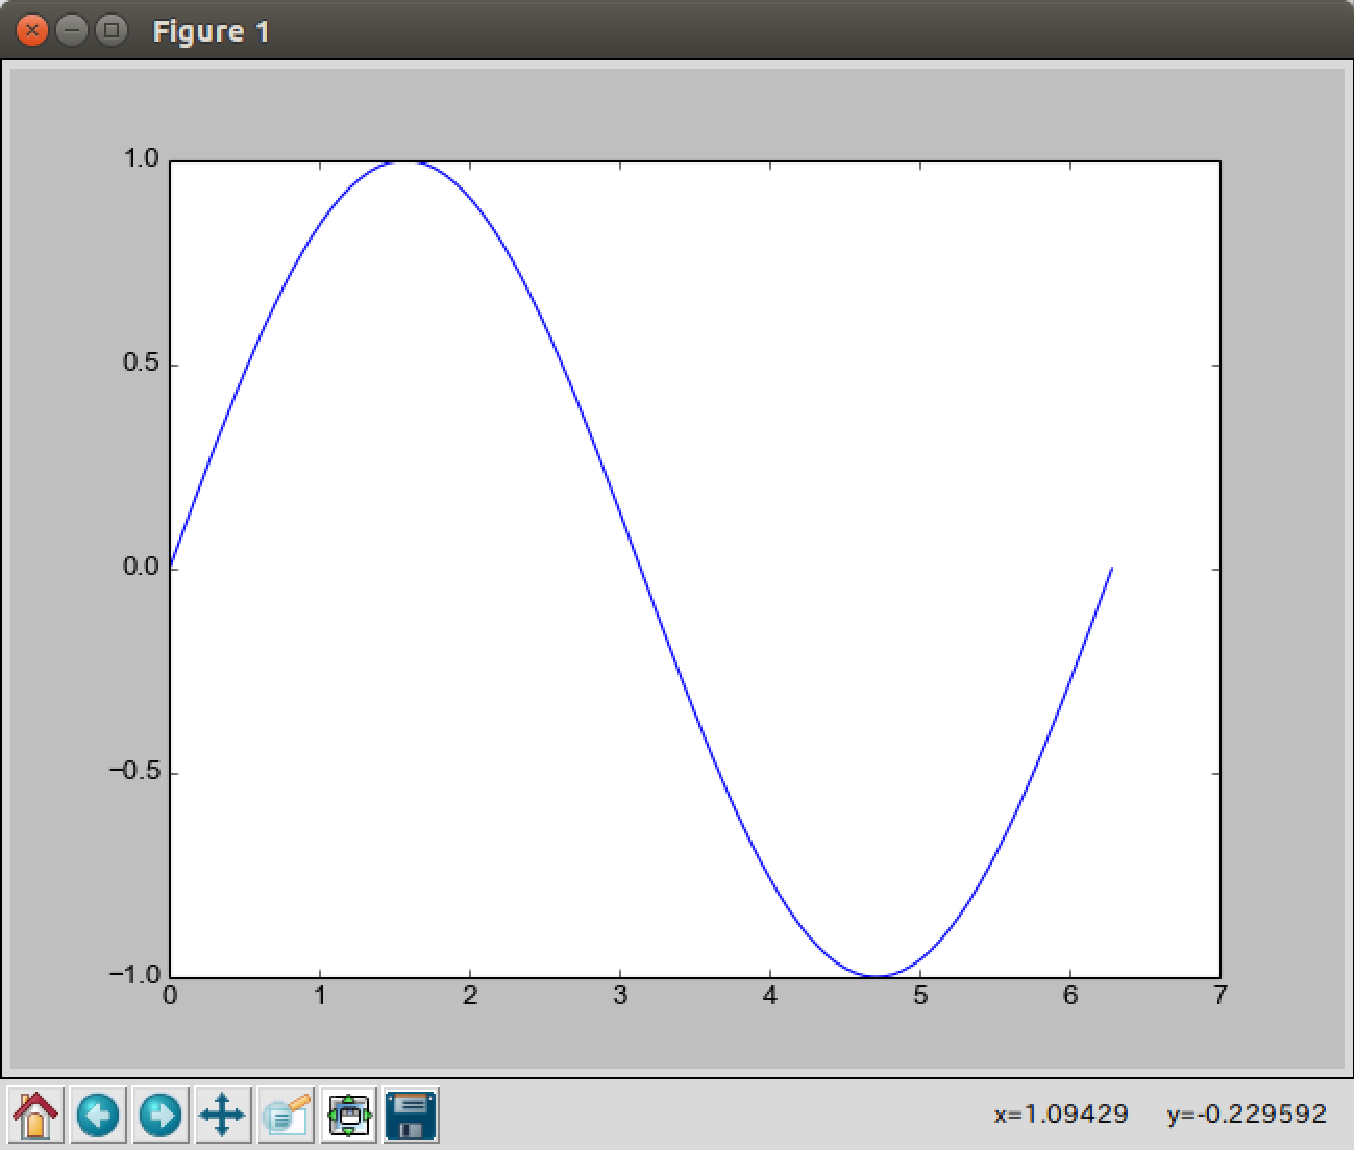
\includegraphics[width=0.3\textwidth]{out/pdf/img/sin.pdf}
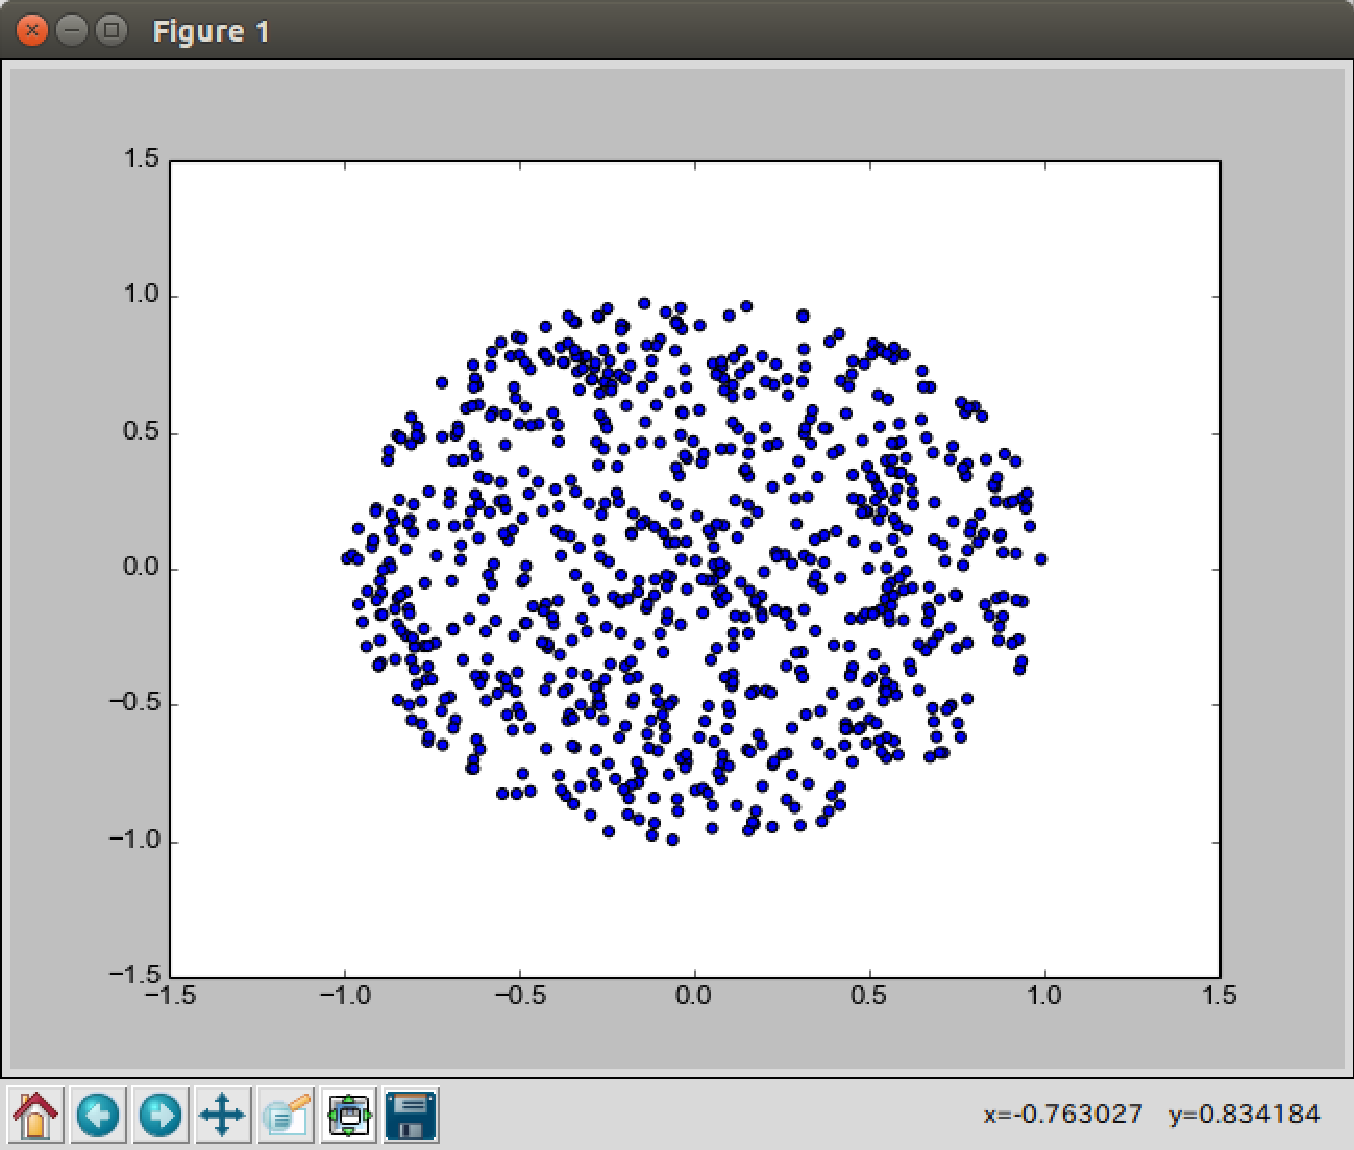
\includegraphics[width=0.3\textwidth]{out/pdf/img/scatter_disc.pdf}
\end{center}

%%%%%%%%%%%%%%%%%%%%%%%%%%%%%%%%%%%%%%%%%%%
\subsection{{\scriptsize matplotlib (2変数の関数)}}
以下をmatplotlibを使って描画してみよ
\begin{enumerate}
\item $z = x^2 - xy + y^2 - x - y$を,$-5\leq x \leq 5$, 
$-5\leq y \leq 5$の範囲で,色で
{\small (データの与え方はスライドもしくはcheet sheet参照)}.
\item 前問題と同じ関数を,ただし3Dの曲面で
\end{enumerate}
\begin{center}
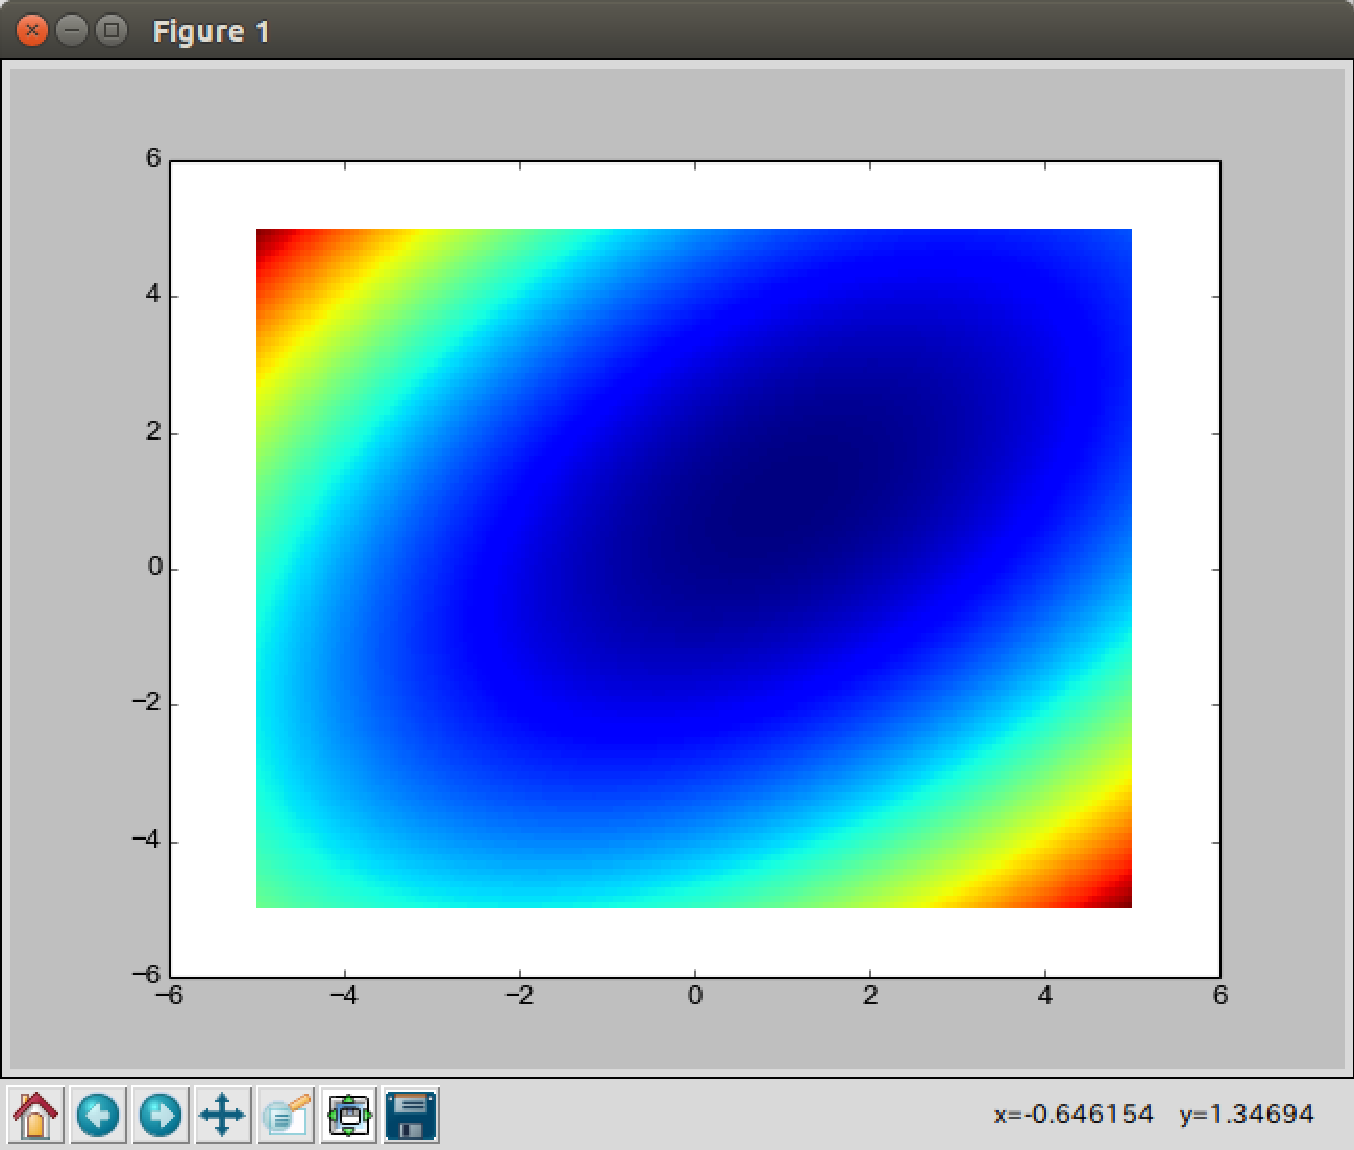
\includegraphics[width=0.3\textwidth]{out/pdf/img/xx_pcolor.pdf}
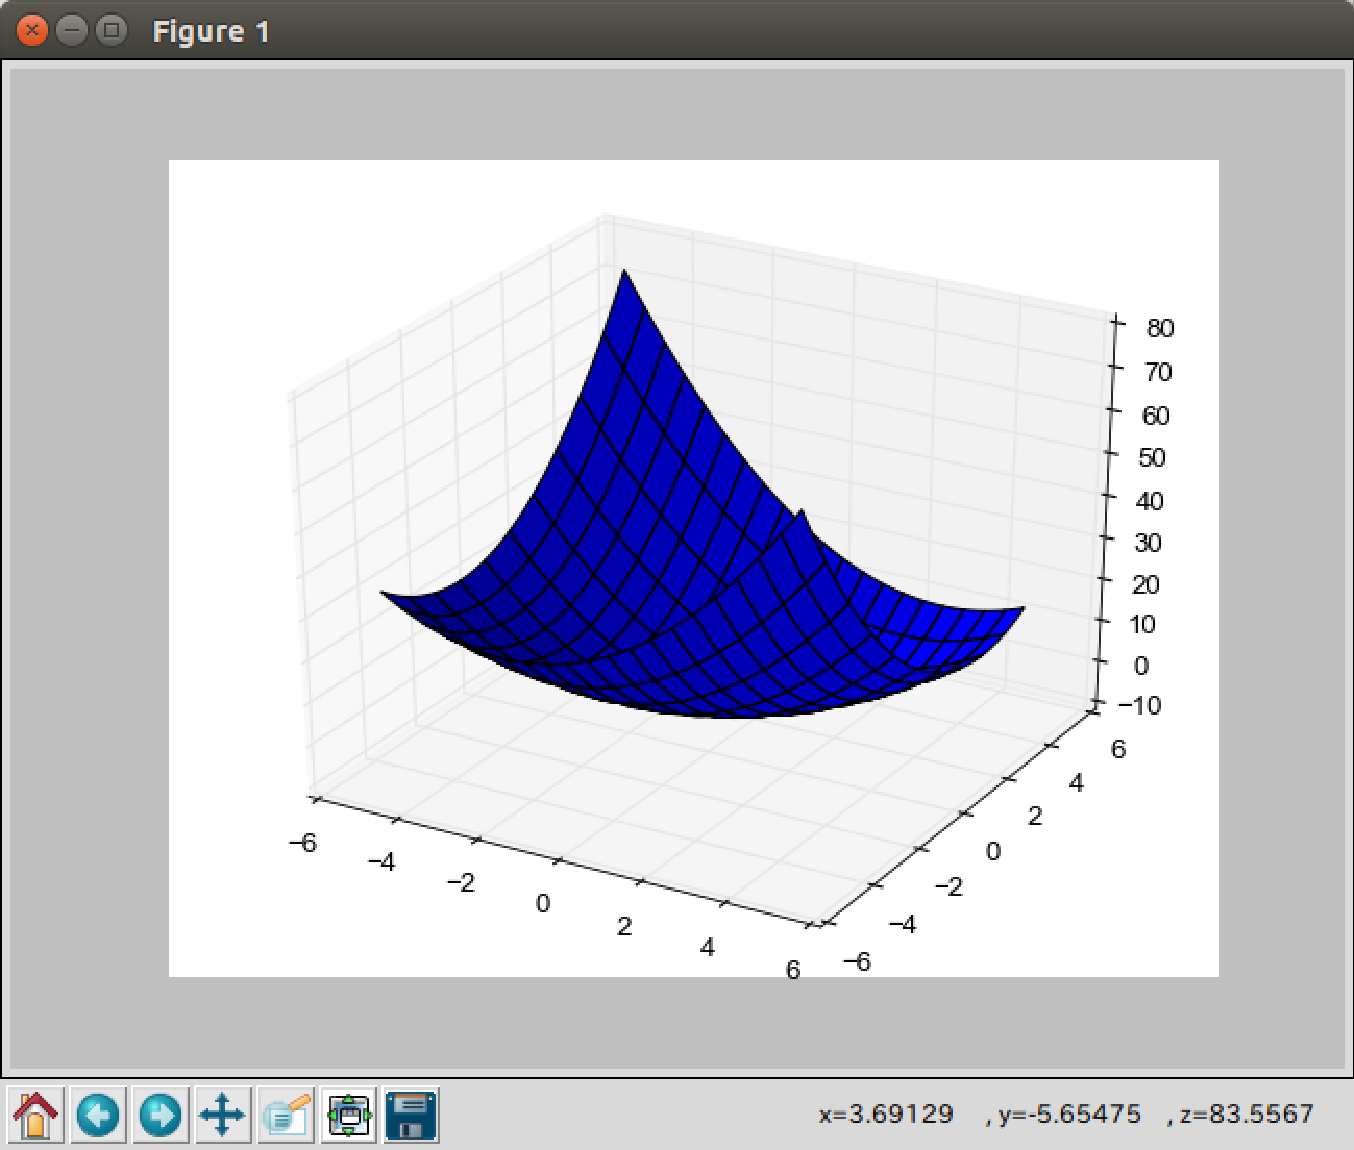
\includegraphics[width=0.3\textwidth]{out/pdf/img/xx_surface.pdf}
\end{center}


\newpage

\section{}

%%%%%%%%%%%%%%%%%%%%%%%%%%%%%%%%%%%%%%%%%%%
\subsection{{\scriptsize 場の方程式}}
$x$と$t$の関数$u(x,t)$に関する偏微分方程式:
\begin{eqnarray*}
\frac{\partial u}{\partial t} & = & 2\, \frac{\partial u}{\partial x} 
\quad (-5 < x < 5) \\
u(x, 0) & = & 
\left\{ 
\begin{array}{ll}
 x + 1 & (-1 \leq x \leq 0) \\
-x + 1 & (0 \leq x \leq 1) \\
0      & (|x| > 1)
\end{array}
\right. \\
u(0, t) & = & 0 \\
u(1, t) & = & 0
\end{eqnarray*}
をシミュレーションしたい.
\begin{enumerate}
\item 初期値$u(x, 0)$をmatplotlibを用いてplotせよ
\item 微分方程式を
$t = 2$までシミュレーションし,結果をmatplotlibを用いてplotせよ
\end{enumerate}

なお,この方程式は手でも解ける.{\bf 任意の}一変数関数
$g(y)$に対し,
\[ u(x, t) = g(x + 2 t) \]
とすれば,
\begin{eqnarray*}
\frac{\partial u}{\partial t} & = & 2\, \frac{\partial u}{\partial x} 
\end{eqnarray*}
が満たされる.$t=0$を代入すると,
\[ u(x, 0) = g(x) \]
すなわち,$g$は初期値そのものである.
つまり,$u(x, t)$は,初期値を$-2t$だけ平行移動したものにすぎない.
すなわち左方向に速さ2で平行移動していくだけである.

%%%%%%%%%%%%%%%%%%%%%%%%%%%%%%%%%%%%%%%%%%%
\subsection{{\scriptsize 場の方程式. 2次元}}
$u$は2次元の座標$(x,y)$と時刻$t$の関数で以下を満たす.
\begin{eqnarray*}
\frac{\partial u}{\partial t} & = & 
\frac{\partial^2 u}{\partial x^2} +
\frac{\partial^2 u}{\partial y^2} 
\quad (0 < x < 1,\, 0 < y < 1) \\
u(x, y, 0) & = & \mbox{適当([0,1]の乱数)} 
\quad (0 < x < 1,\, 0 < y < 1) \\
u(x, 0, t) & = & x \\
u(1, y, t) & = & 1 \\
u(x, 1, t) & = & 1 \\
u(0, y, t) & = & y \\
\end{eqnarray*}
をシミュレーションしたい.

\begin{enumerate}
\item 初期状態をmatplotlibを使って色で可視化(pcolor)せよ
\item 十分大きな$t$までシミュレートした結果を,
をmatplotlibを使って可視化せよ
\end{enumerate}


\end{document}

\newpage
\section{}


\newpage
\section{}

%%%%%%%%%%%%%%%%%%%%%%%%%%%%%%%%%%%%%%%%%%%
\subsection{{\scriptsize (乱数)}}
randomというモジュールをimportすると, random()という関数が
使える. これは, 区間[0,1]から数をひとつランダムに生成する.
\begin{itemize}
\item []
\begin{lstlisting}
import random
random.random()
@\resa{0.8408639918721788}@
random.random()
@\resa{0.7644349032373015}@
random.random()
@\resa{0.6271941721108247}@
\end{lstlisting} % $
\end{itemize}

乱数を用いて, 箱 $[-1,1] \times [-1,1] \times [-1,1]$に
多数の点を発生させ,visual pythonで可視化してみよ.
例えば,

\begin{itemize}
\item 原点からの距離 $\leq$ 1.0 ならば黄色で大きめに表示
\item そうでなければ白で小さめに表示
\end{itemize}
とかやって,こんなアート(??)\footnote{本物のアートをやっている人,ごめんなさい}を作ってみよう
(今までの知識でできることをやってみているだけで,アートはなんでもよい).

\begin{center}
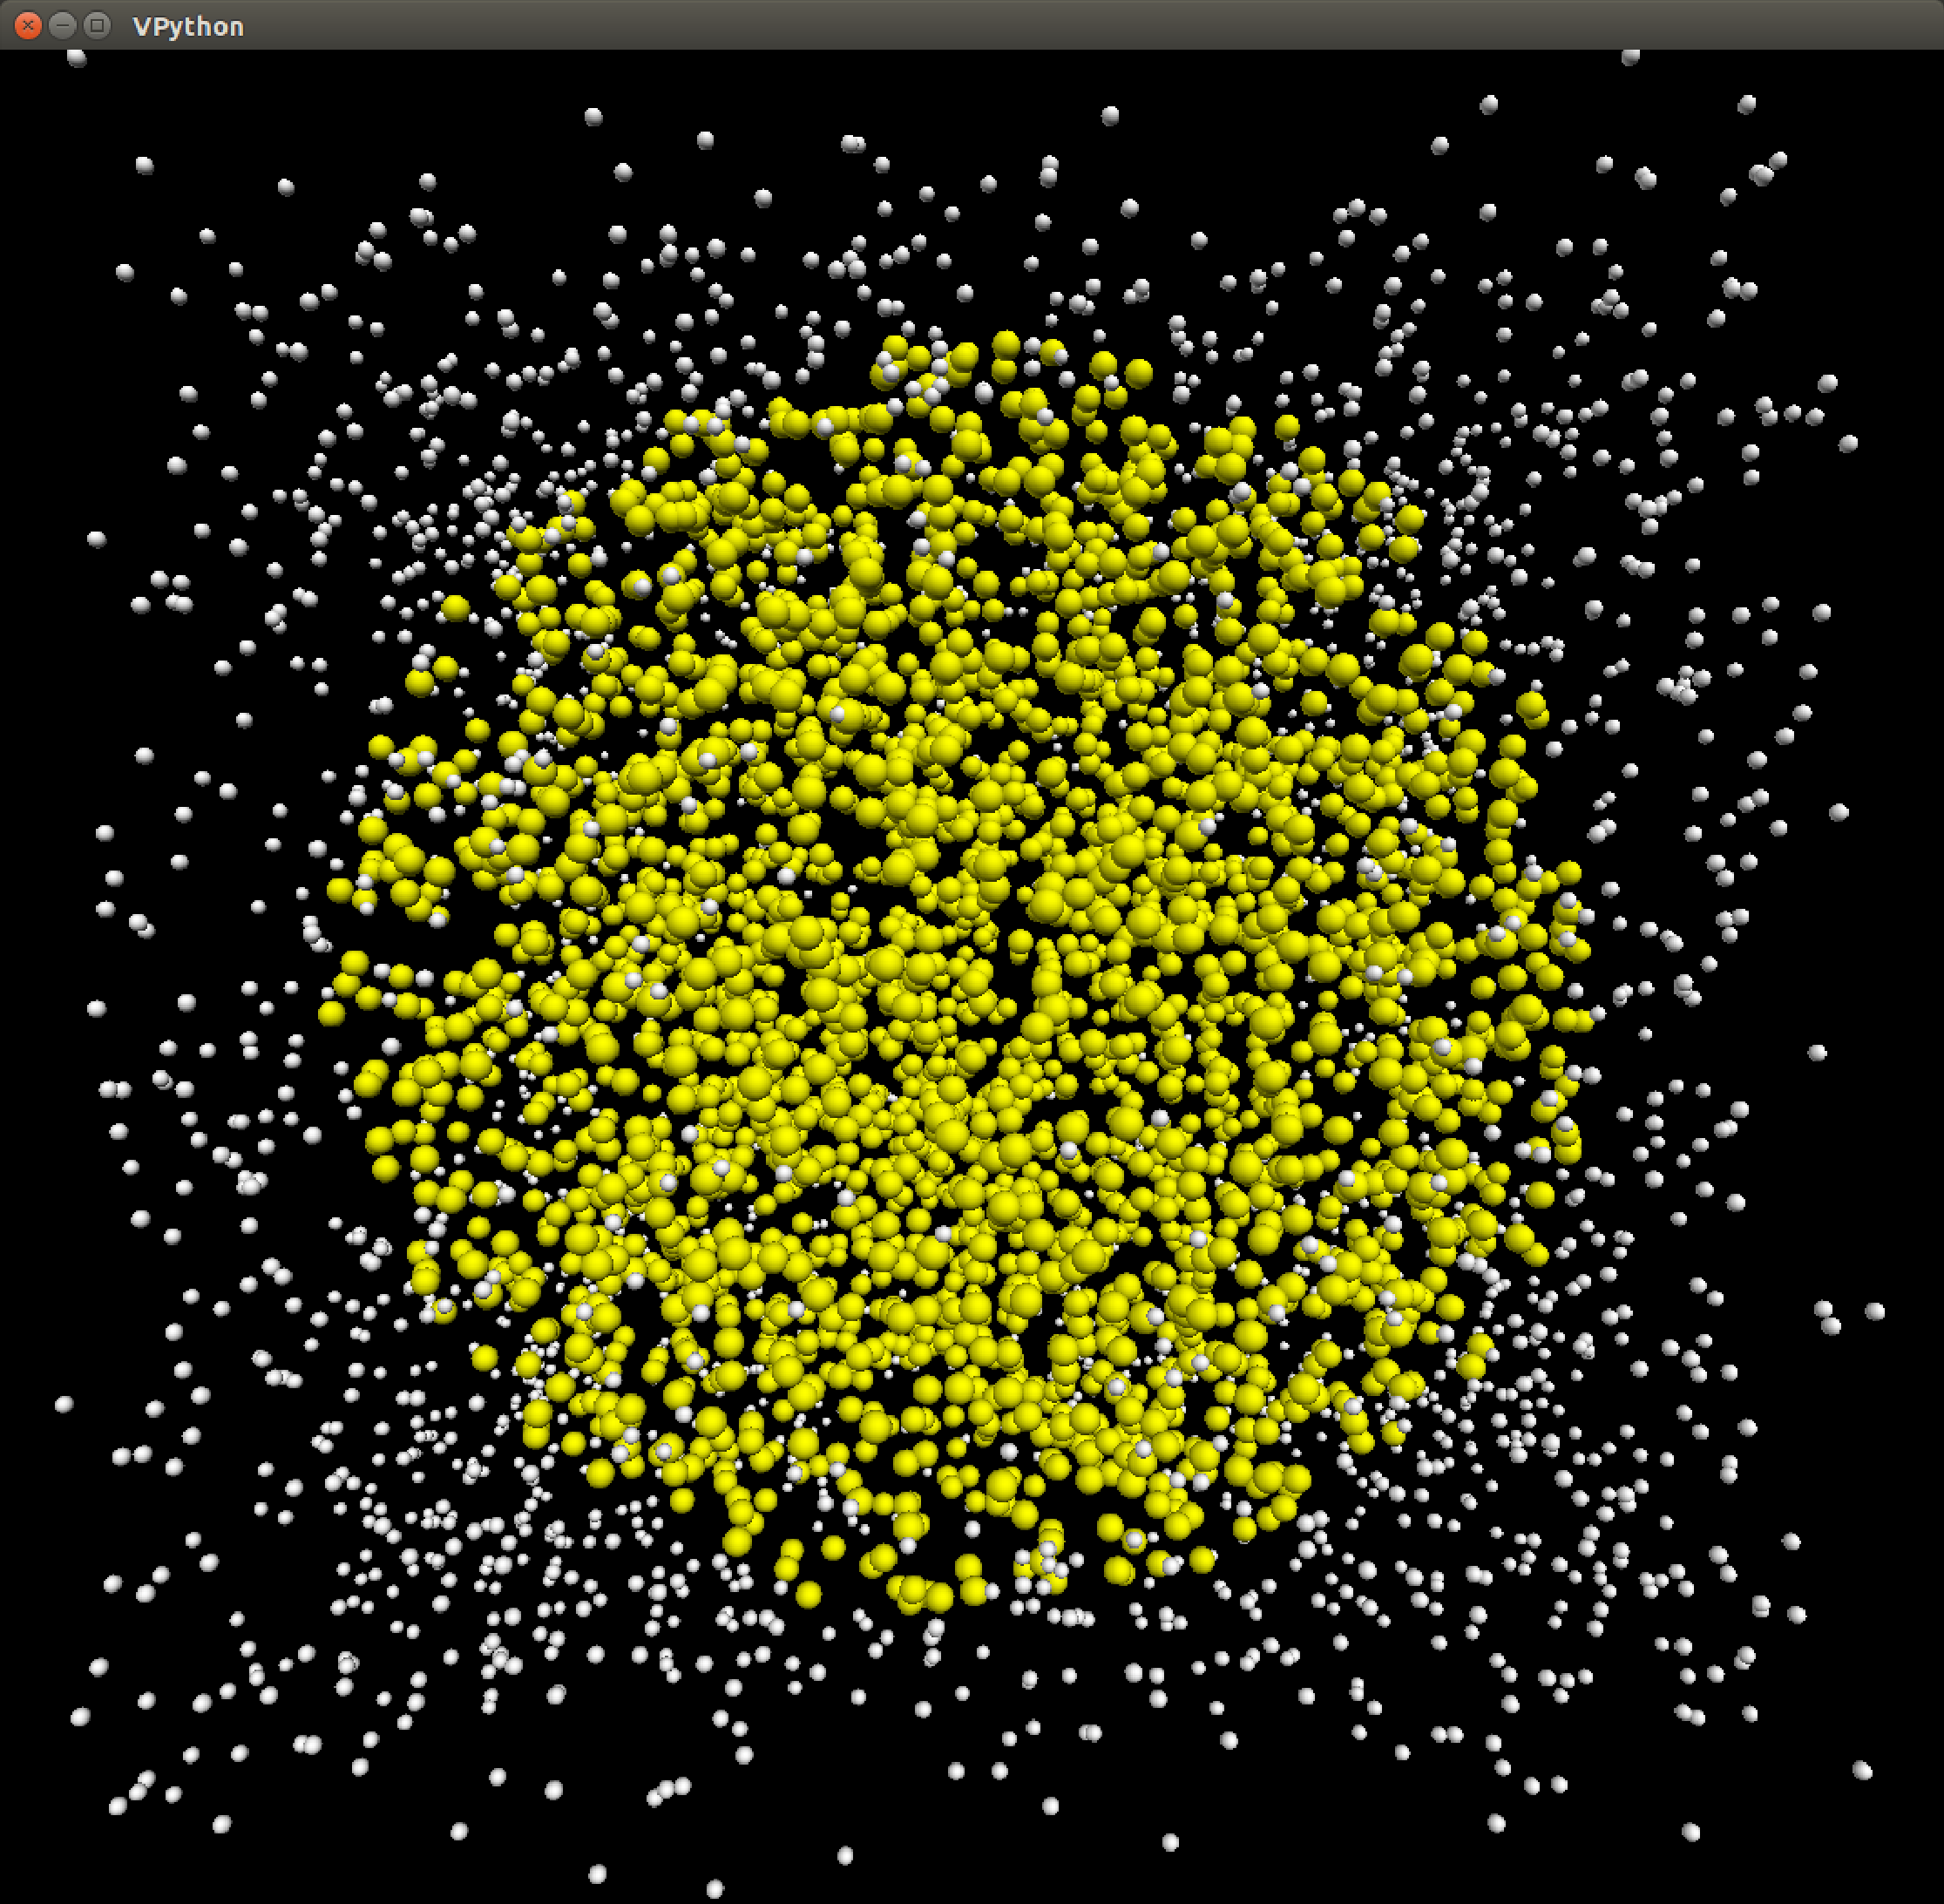
\includegraphics[width=0.3\textwidth]{out/pdf/img/art.pdf}
\end{center}

%%%%%%%%%%%%%%%%%%%%%%%%%%%%%%%%%%%%%%%%%%%
\subsection{{\scriptsize (乱数)}}
前問の関数を少し変更し,$n$を与えられると,
$n$個の点を発生させ,
\[ \frac{\mbox{「原点からの距離} \leq \mbox{1.0」の点の数}}{n} \]
を計算する関数を書け.十分大きな$n$を与えると,
この値はどのような値になるはずか?

これは,計算機で積分を計算する方法,
特に多次元の積分を計算する強力な方法を与える.
\ref{subsec:integrate}でやったように,
積分区間を等分するのも方法だが,多次元になると急激に点の数が増えてしまう.

%%%%%%%%%%%%%%%%%%%%%%%%%%%%%%%%%%%%%%%%%%%
\iffalse
\subsection{{\scriptsize 乱数は確率の問題を解く基本かつ最強の武器}}
モンティ・ホール問題という, TV番組で物議をかもした問題が有る.

ゲームのルール(Wikipediaより):
\begin{enumerate}
\item 3つのドア (A, B, C) に(景品、ヤギ、ヤギ)がランダムに入っている。
\item プレイヤーはドアを1つ選ぶ。(プレイヤーはドアの中身を知らない)
\item モンティは残りのドアのうち1つを必ず開ける。
\item モンティの開けるドアは、必ずヤギの入っているドアである。
(モンティはドアの中身を知っている)
\item モンティはプレーヤーにドアを選びなおしてよいと必ず言う。 
\end{enumerate}
このときプレイヤーはドアを選び直したほうが良いのか?

という問題.

乱数を使ったシミュレーションを行い「選びなおす」
「選び直さない」それぞれのケースで,景品をひく確率を求めよ.

こうして正解がわかるという話と,納得しない人をどう納得させるかというのは別の話ですがw
\fi


\newpage
\section{}

%%%%%%%%%%%%%%%%%%%%%%%%%%%%%%%%%%%%%%%%%%%
\subsection{{\scriptsize (リスト内包表記)}}
リスト内包表記を使って以下の関数を, 
「1行で」書いてみよう(「行数」には,関数の本体のみを数える.
必要なimport文や,関数のヘッダ行({\tt def f(x,y):} の行)は含まない).

\begin{enumerate}
\item リスト$L$と数$a$を受け取り,
$L$の各要素に$a$を足したリストを返す関数({\tt add}).
動作例:
\begin{itemize}
\item []
\begin{lstlisting}
>>> add([5,3,8], 4) 
[9,7,12]
\end{lstlisting}
\end{itemize}

\item $n$が与えられ
\[ 1^3 + 2^3 + \cdots + n^3 \]
を返す関数. 以前ならループで以下のように書いたものだが,
リスト内包表記を使うと?
\begin{itemize}
\item []
\begin{lstlisting}
def sum_cube(n):
    s = 0
    for i in range(1, n+1):
        s = s + i ** 3
    return s
\end{lstlisting}
\end{itemize}

\item 同じ長さのリスト$X$, $Y$を受け取り,
それぞれをベクトルとみなした時の内積を返す関数
(ヒント: zipという関数がある).
動作例:
\begin{itemize}
\item []
\begin{lstlisting}
>>> dot([1,2,3,4], [4,5,6,7]) 
60
\end{lstlisting}
\end{itemize}

\item 2つの実数$a, b$と整数$n \geq 2$を受け取り,
  $[a,b]$を$(n-1)$等分する$n$点(両端の$a$と$b$を含む)
  をリストにして返す関数
(注: numpyにはまさしくそのような関数{\tt linspace($a, b, n$)}がある)
動作例:
\begin{itemize}
\item []
\begin{lstlisting}
>>> linspace(1.0, 2.0, 5)
[ 1.0, 1.25, 1.5, 1.75, 2.0 ]
\end{lstlisting}
\end{itemize}

\item 前回作った積分関数を,リスト内包表記で1-2行で書いてみよ.
\end{enumerate}

\newpage

\section{}
%%%%%%%%%%%%%%%%%%%%%%%%%%%%%%%%%%%%%%%%%%%
\subsection{{\scriptsize 初めての物理シミュレーション(1)}}
ボールの初期速さと投射角が与えられる.
その後のボールの軌道をシミュレートし,
Visual Pythonを用いてアニメーションせよ.
ボールには重力だけが働くものとする.

\begin{enumerate}
\item まずは一つのボールのアニメーションをせよ. 
  時間の刻み幅や, 繰り返し回数は, 
  まずは適当(100回とか)に決め,
  できたら地面に着地すると終わるように
  (hint: for文を終了するのにbreak文を使う)するとよい.
\begin{itemize}
\item []
\begin{lstlisting}
def free_fall(v0, theta):
    ...    
\end{lstlisting}
\end{itemize}
注: Visual Pythonの自動ズーム機能により,
わかりやすいアニメーションにならない場合があるので注意.
例えば十分な長さの$x$軸, $y$軸を表示すると実質的に視点は動かなくなる.

\item ボールの軌跡を表示せよ.Visual Pythonのcurveという
オブジェクトを使うと良い.

\item $^\ast$ 余力があれば,
  色々な角度(リストで与えられる)で発射されたボールを同時に,
  軌跡と共にアニメーションせよ.
  ボールのリストを作り,各ボールを一ステップずつ進める.
  よく知られているように45度が一番遠くまで飛ぶはずである.
\end{enumerate}

\begin{center}
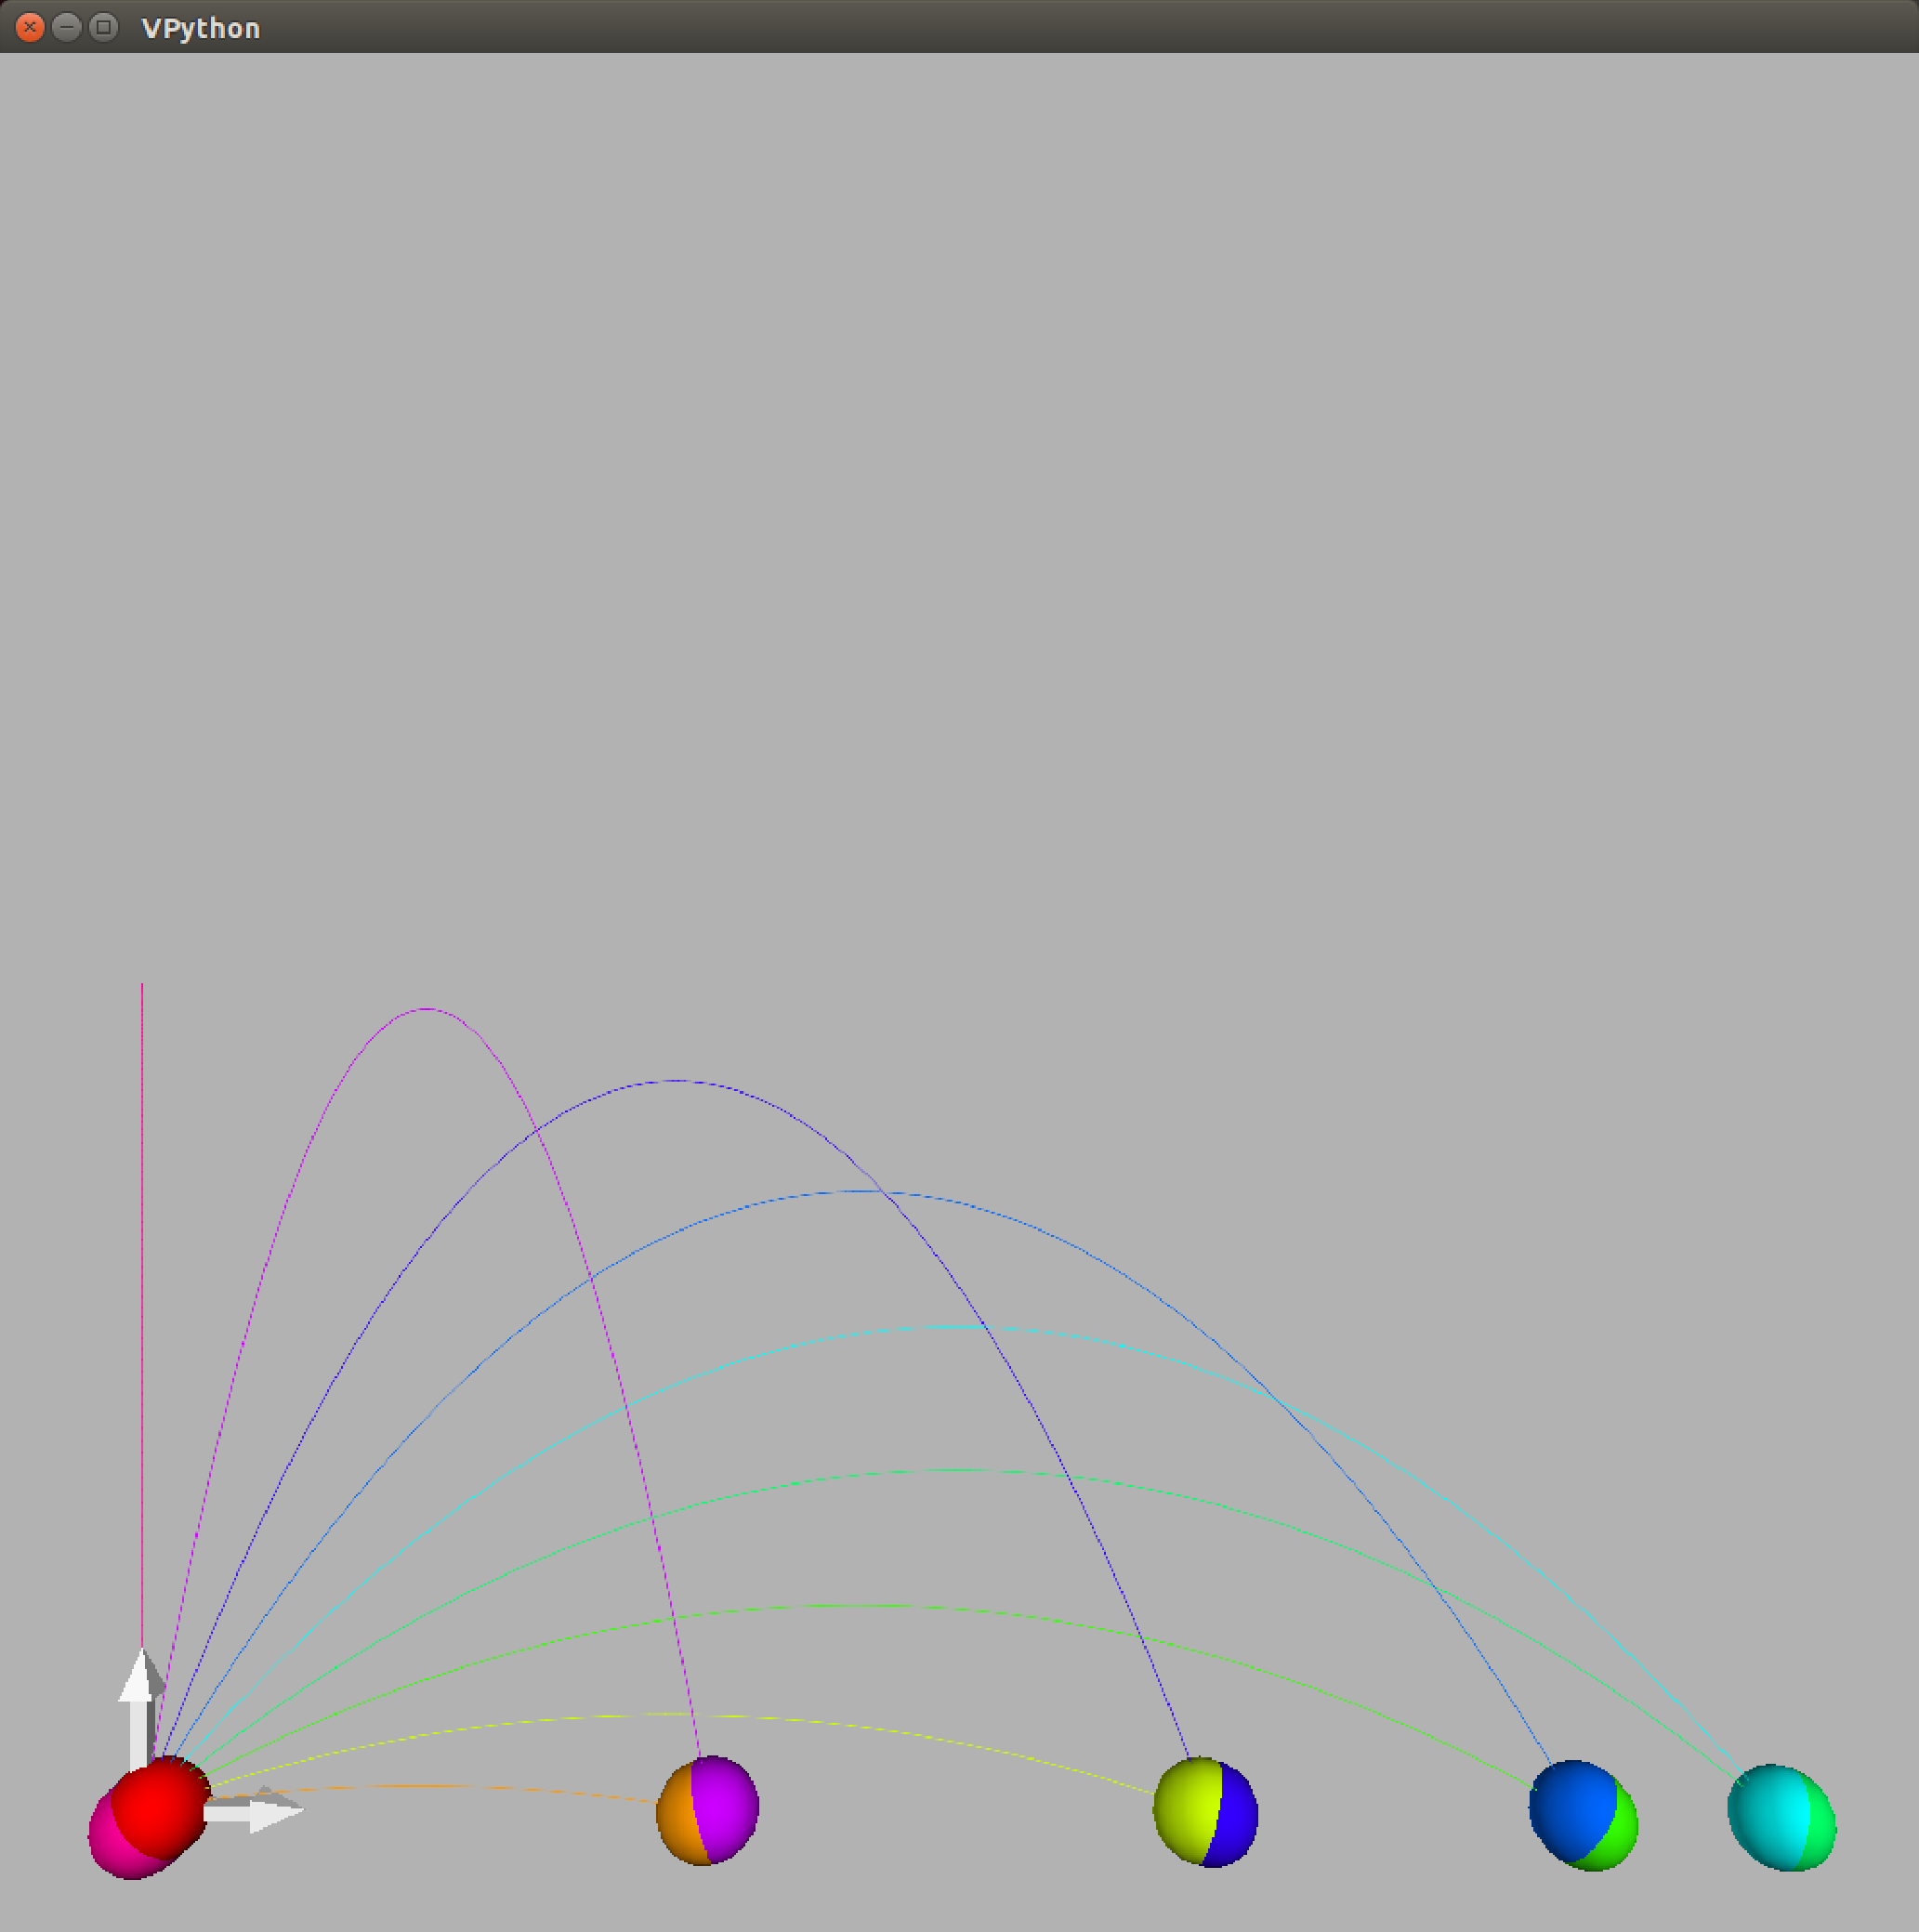
\includegraphics[width=0.4\textwidth]{out/pdf/img/para.pdf}
\end{center}

\newpage

%%%%%%%%%%%%%%%%%%%%%%%%%%%%%%%%%%%%%%%%%%%
\subsection{{\scriptsize 初めての物理シミュレーション(2)}}
二つの質点の質量,初期位置,初期速度が与えられる.
その後の動きをVisual Pythonを用いてアニメーションせよ.
二つの質点の間には, 両者の質量を$m_0$, $m_1$, 
両者の間の距離を$r$として大きさ
\[ \frac{m_0 m_1}{r^2} \]
の引力が働くものとする(方向は2体を結ぶ方向). 
いわゆる万有引力定数を省略している.
運動の定性的な理解に影響がないことは直感的には頷けると思うが,
それが1になるように単位(質量や長さ)
の中に組み込まれていると考えれば良い.

\begin{enumerate}
\item まずは適当に時間の刻み幅と回数を決め,アニメーションせよ.
\begin{itemize}
\item []
\begin{lstlisting}
def two_bodies(m0, x0, v0, m1, x1, v1):
    ...
\end{lstlisting}
\end{itemize}
\item 質点の軌跡を表示せよ(curveオブジェクトを使う).

\item 各ステップで, 以下の3つの値を表示せよ
  \begin{itemize}
  \item $K = $ 運動エネルギーの和
  \item $U = $ ポテンシャルエネルギー
  \item $K + U$ 
  \end{itemize}
ただし,
\[ U = - \frac{m_0 m_1}{r} \]

\item $^\ast$ 余力があれば(時間が余ってしまった人は), 
適当に$n$個の点(質量, 初期位置, 初速度)
を生成し, その$n$個の点の動きをアニメーションせよ.
軌跡は表示しないほうがよいでしょう.
ポテンシャルエネルギーは上記を全ペアに対して足したもの.

\end{enumerate}

\begin{center}
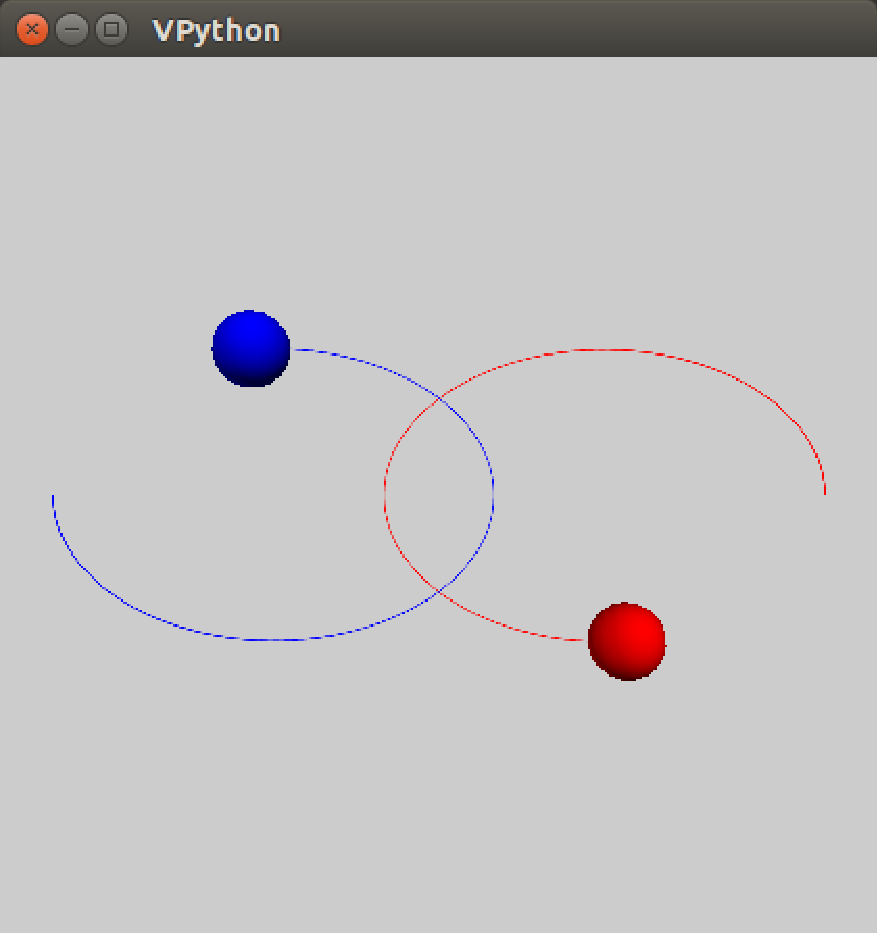
\includegraphics[width=0.4\textwidth]{out/pdf/img/two_bodies.pdf}
\end{center}

\newpage

%%%%%%%%%%%%%%%%%%%%%%%%%%%%%%%%%%%%%%%%%%%
\subsection{{\scriptsize 初めての物理シミュレーション(3)}}
バネで吊るされた質点に,時間と共に変わる外力 $f(t)$:
を与えたときの運動をVisual Pythonを用いてアニメーションせよ
($t$は時刻,$f(t)$は垂直方向のベクトル).
バネ定数$k$, 質点の質量が$m$で,
初期状態は自然長の位置に停止しているとする.

\begin{enumerate}
\item 外力が0のときの動きをアニメーションせよ.
\begin{itemize}
\item []
\begin{lstlisting}
def spring(k, m, f):
    ...  
\end{lstlisting}
\end{itemize}
バネはhelixオブジェクトを使うと表示できる.

\item 外力が,
\[ f(t) = \sin \omega t \]
の時の様子をシミュレーションせよ.
$\omega$がある値だと質点の動きは大きくなる.
それはいくらか,数学の知識でわかる人はその値を試してみよ.
わからなければ色々やってみよ.

\end{enumerate}

\begin{center}
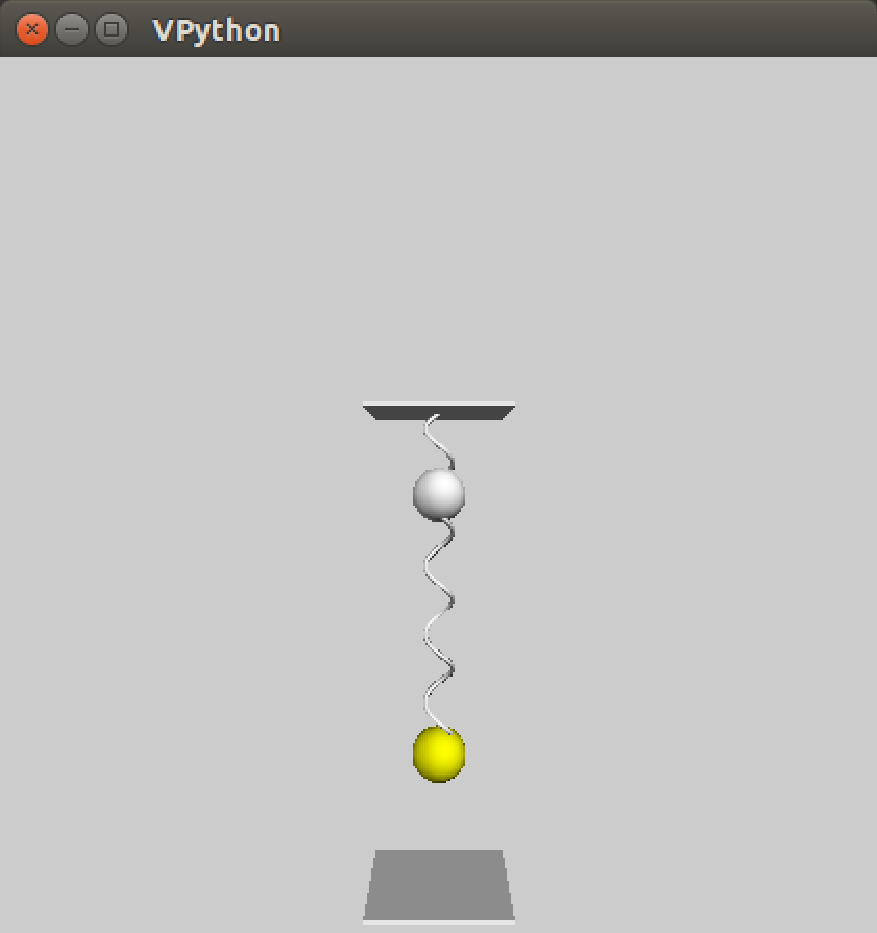
\includegraphics[width=0.4\textwidth]{out/pdf/img/spring.pdf}
\end{center}


\newpage

\section{}

%%%%%%%%%%%%%%%%%%%%%%%%%%%%%%%%%%%%%%%%%%% 
\subsection{{\scriptsize matplotlib (1変数の関数)}}
以下をmatplotlibを使って描画してみよ
\begin{enumerate}
\item 最もプリミティブな確認. リストだけを使って,
点 $(1,1)$, $(2,4)$, $(3,9)$, $(4,16)$をつないだグラフ
\item $y = \sin(x)$のグラフを$0 \leq x \leq 2\pi$の範囲で
{\small (numpyの機能をかっこよく使って)}.
\item $x^2 + y^2 \leq 1$の範囲にランダムにばらまかれた点
{\small (plotの代わりにscatter)}.
\end{enumerate}

\begin{center}
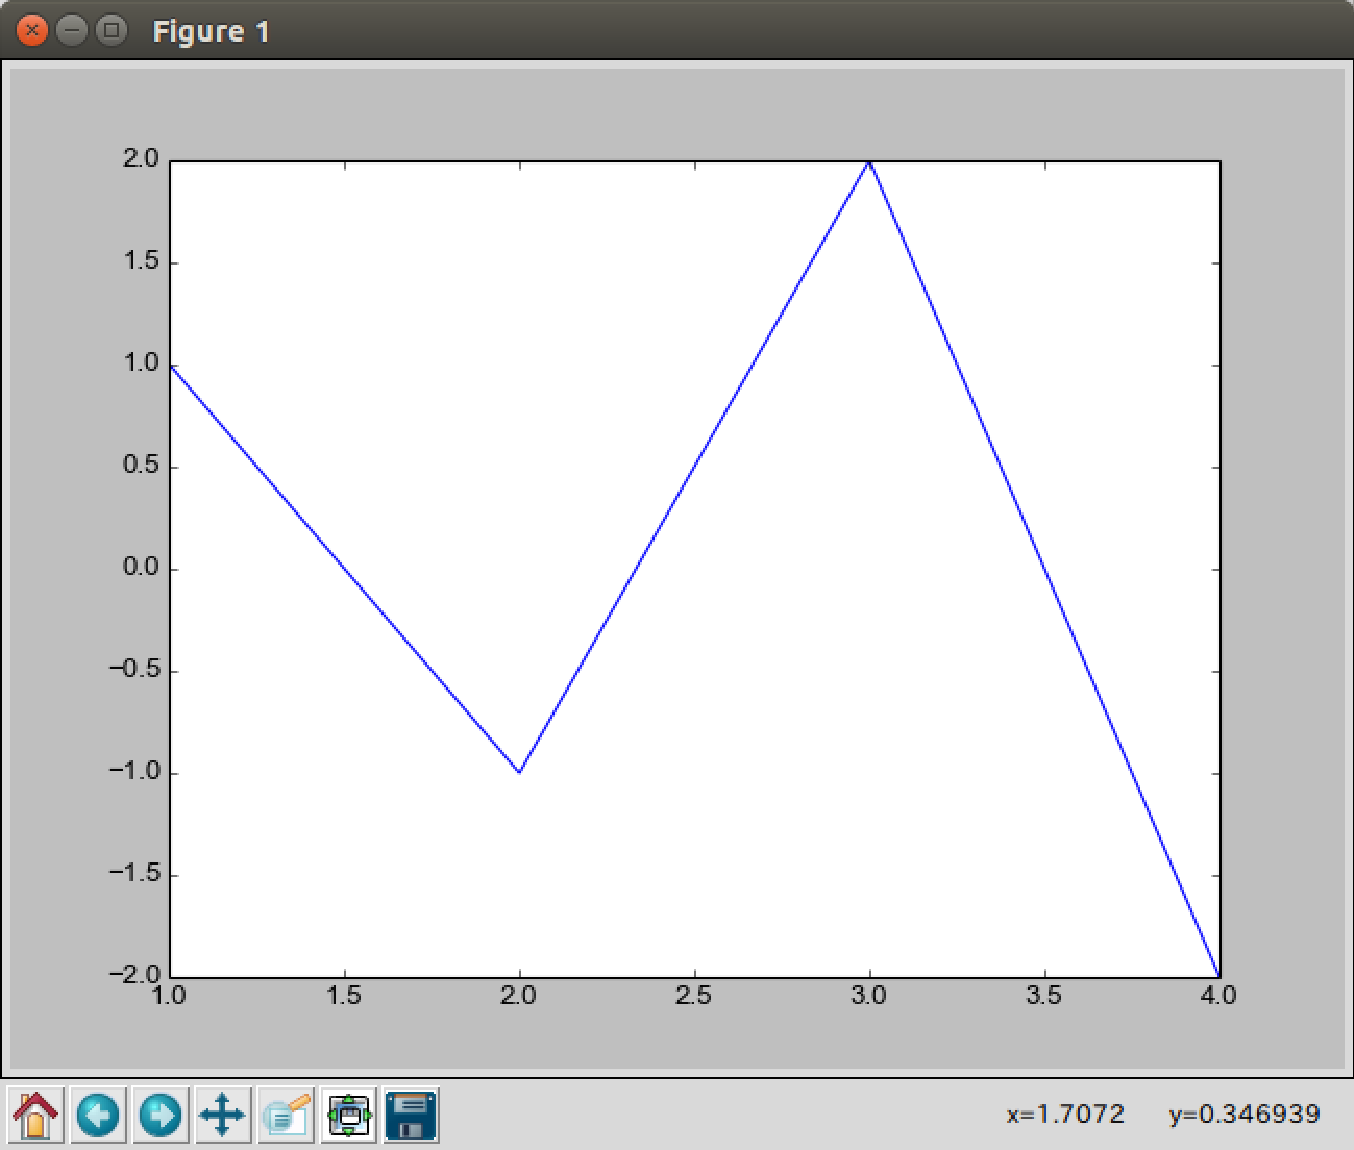
\includegraphics[width=0.3\textwidth]{out/pdf/img/plot_practice.pdf}
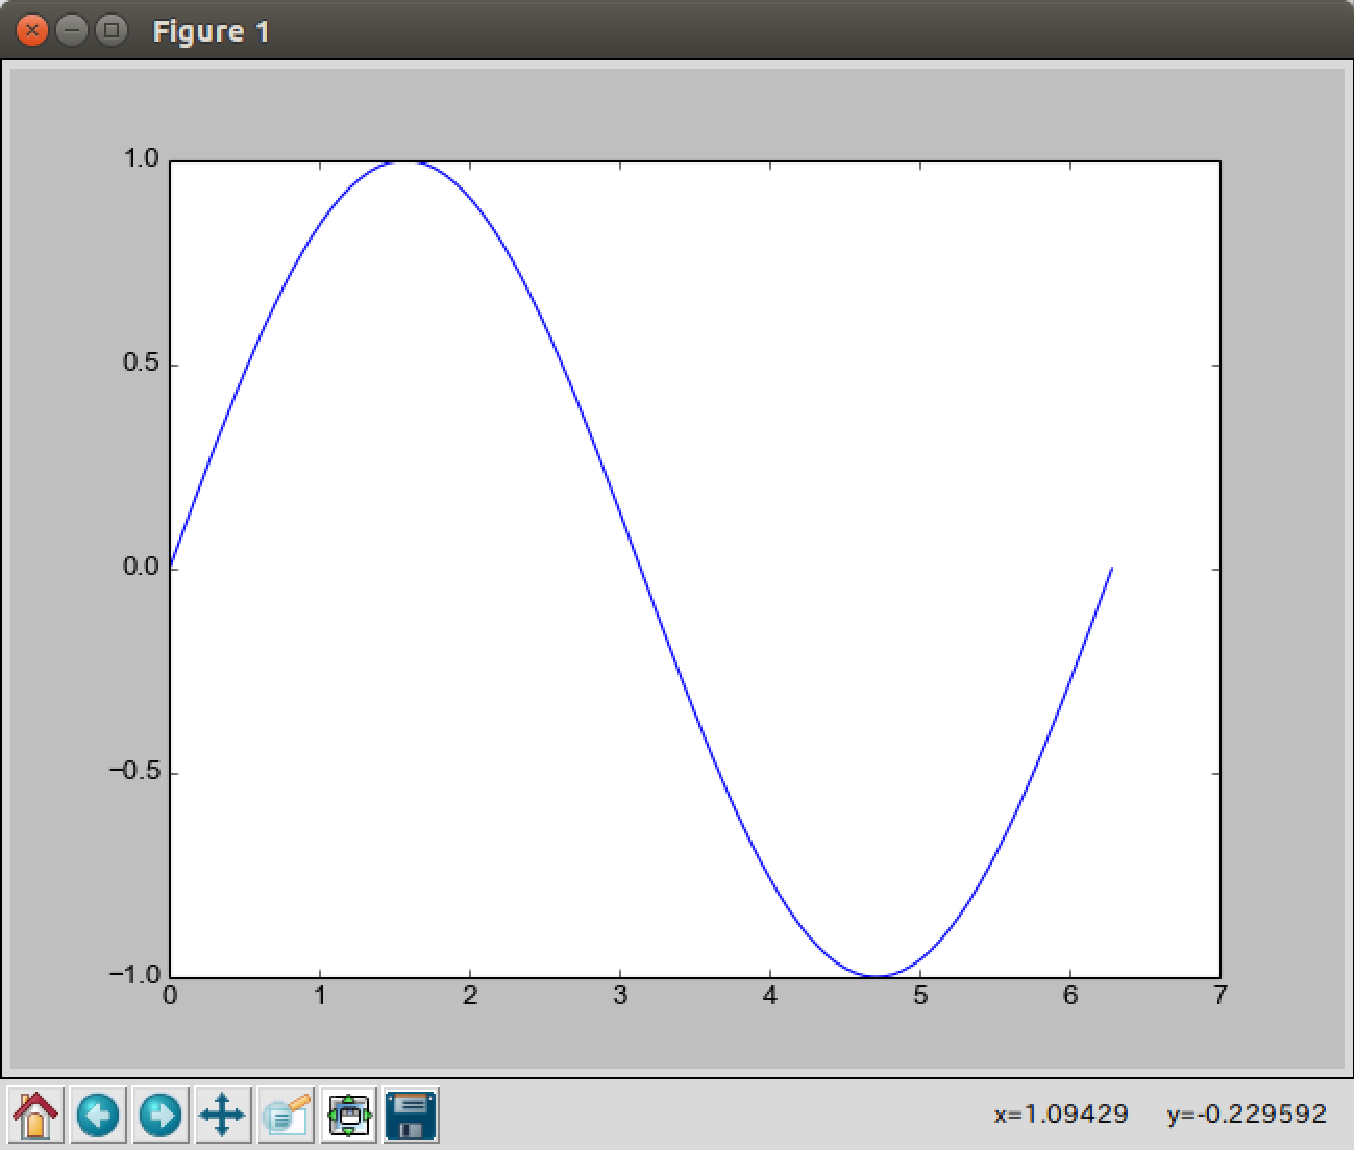
\includegraphics[width=0.3\textwidth]{out/pdf/img/sin.pdf}
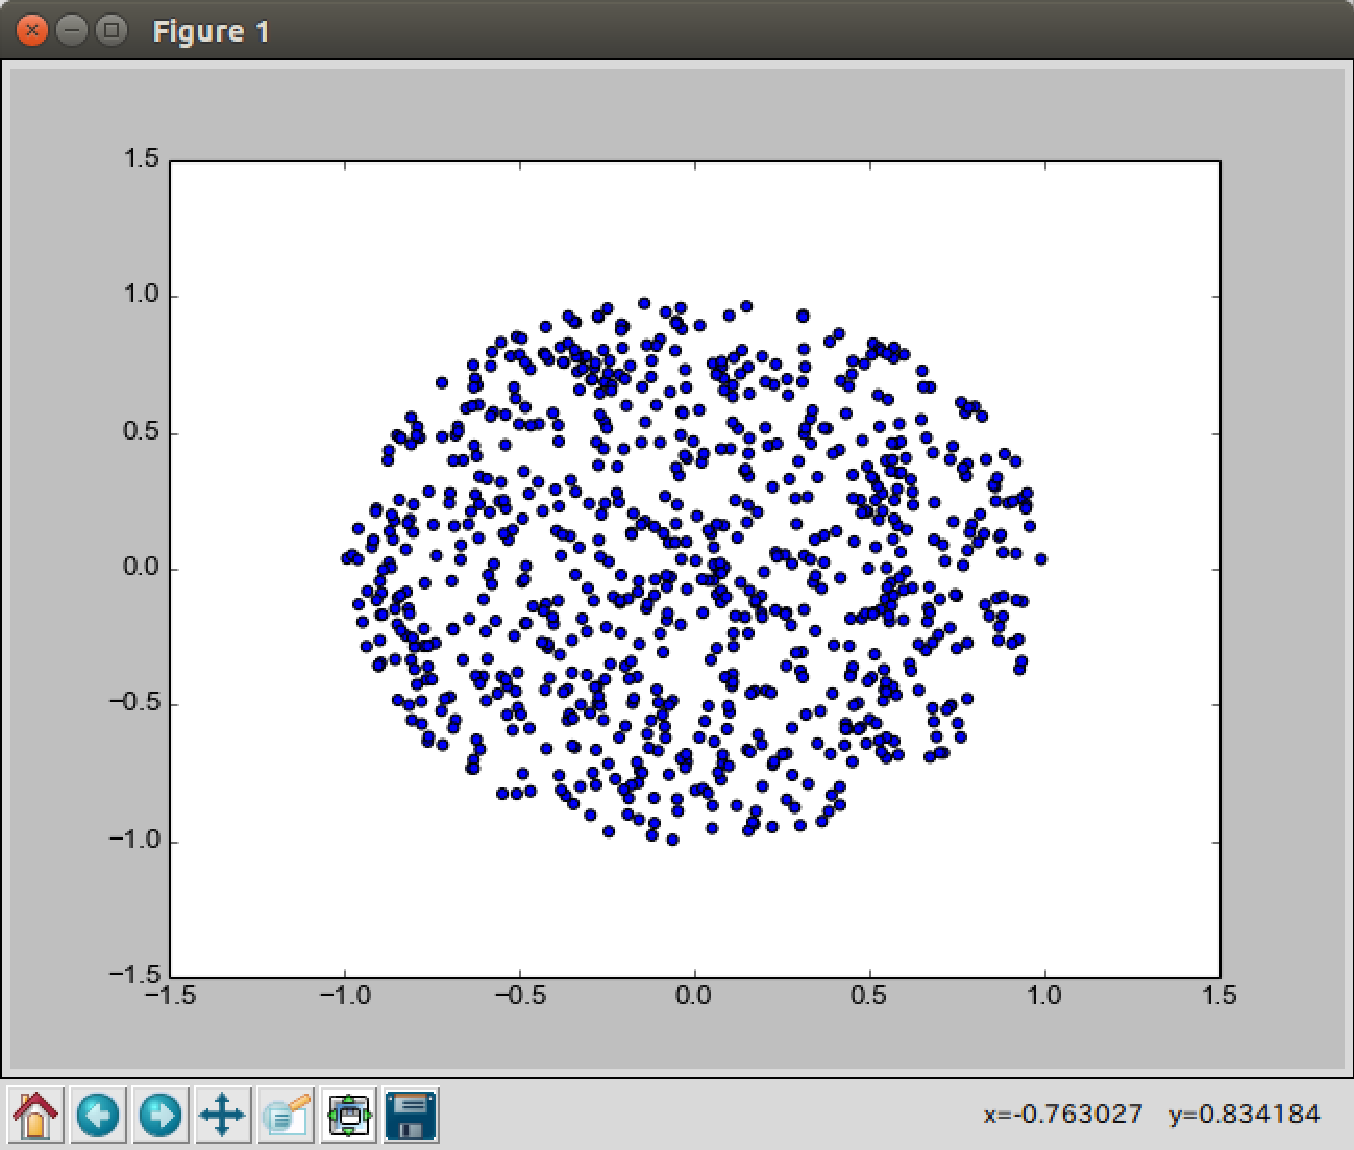
\includegraphics[width=0.3\textwidth]{out/pdf/img/scatter_disc.pdf}
\end{center}

%%%%%%%%%%%%%%%%%%%%%%%%%%%%%%%%%%%%%%%%%%%
\subsection{{\scriptsize matplotlib (2変数の関数)}}
以下をmatplotlibを使って描画してみよ
\begin{enumerate}
\item $z = x^2 - xy + y^2 - x - y$を,$-5\leq x \leq 5$, 
$-5\leq y \leq 5$の範囲で,色で
{\small (データの与え方はスライドもしくはcheet sheet参照)}.
\item 前問題と同じ関数を,ただし3Dの曲面で
\end{enumerate}
\begin{center}
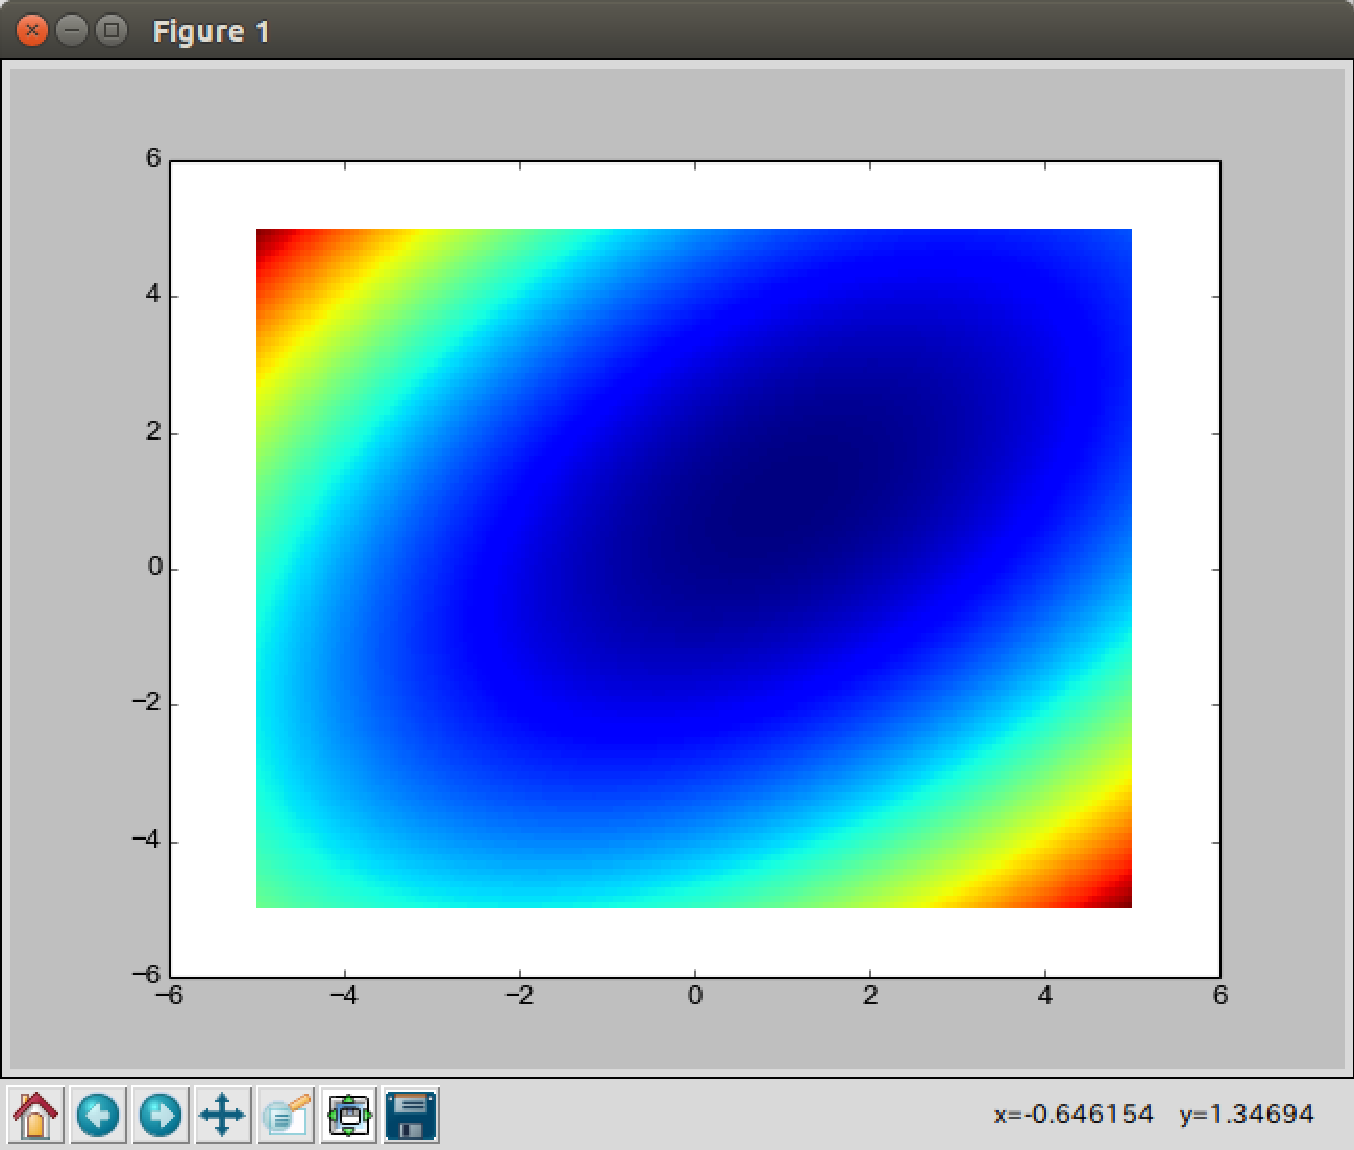
\includegraphics[width=0.3\textwidth]{out/pdf/img/xx_pcolor.pdf}
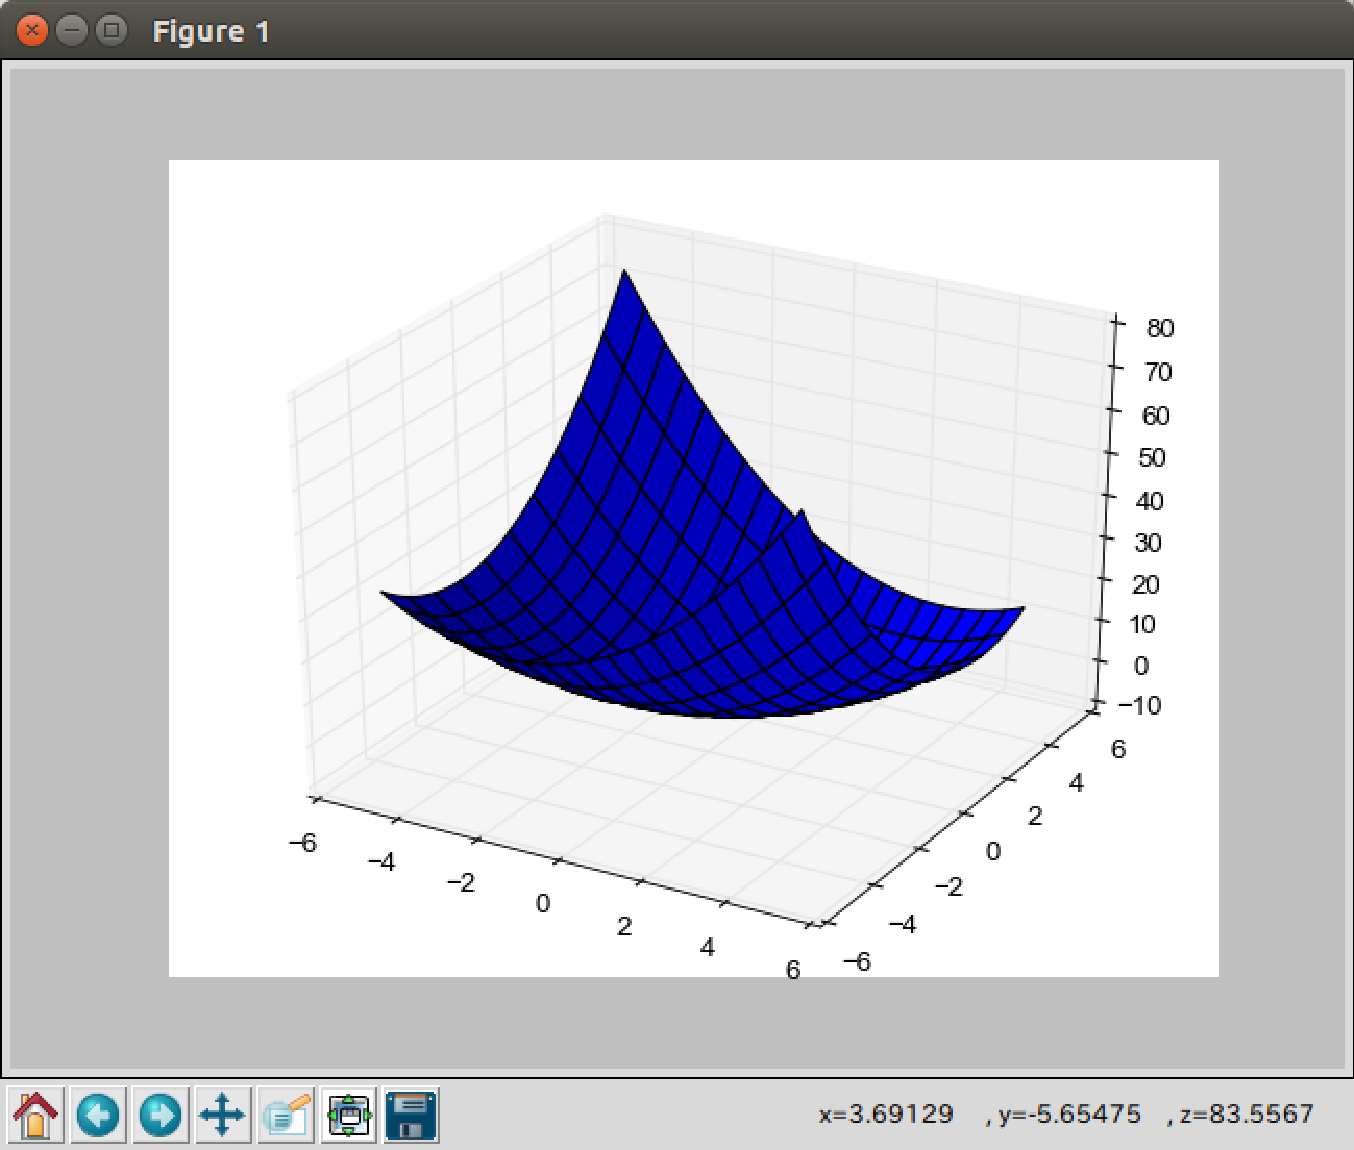
\includegraphics[width=0.3\textwidth]{out/pdf/img/xx_surface.pdf}
\end{center}

\newpage

\section{}

%%%%%%%%%%%%%%%%%%%%%%%%%%%%%%%%%%%%%%%%%%%
\subsection{{\scriptsize 場の方程式}}
偏微分方程式:
\begin{eqnarray*}
\frac{\partial u}{\partial t} & = & 2\, \frac{\partial u}{\partial x} 
\quad (-5 < x < 5) \\
u(x, 0) & = & 
\left\{ 
\begin{array}{ll}
 x + 1 & (-1 \leq x \leq 0) \\
-x + 1 & (0 \leq x \leq 1) \\
0      & (|x| > 1)
\end{array}
\right. \\
u(0, t) & = & 0 \\
u(1, t) & = & 0
\end{eqnarray*}
をシミュレーションしたい
\begin{enumerate}
\item 初期値$u(x, 0)$をmatplotlibを用いてplotせよ
\item 微分方程式を
$t = 2$までシミュレーションし,結果をmatplotlibを用いてplotせよ
\end{enumerate}

なお,この方程式は手でも解ける.{\bf 任意の}一変数関数
$g(y)$に対し,
\[ u(x, t) = g(x + 2 t) \]
とすれば,
\begin{eqnarray*}
\frac{\partial u}{\partial t} & = & 2\, \frac{\partial u}{\partial x} 
\end{eqnarray*}
が満たされる.$t=0$を代入すると,
\[ u(x, 0) = g(x) \]
すなわち,$g$は初期値そのものである.
つまり,$u(x, t)$は,初期値を$-2t$だけ平行移動したものにすぎない.
すなわち左方向に速さ2で平行移動していくだけである.

%%%%%%%%%%%%%%%%%%%%%%%%%%%%%%%%%%%%%%%%%%%
\subsection{{\scriptsize 場の方程式. 2次元}}
$u$は2次元の座標$(x,y)$と時刻$t$の関数で以下を満たす.
\begin{eqnarray*}
\frac{\partial u}{\partial t} & = & 
\frac{\partial^2 u}{\partial x^2} +
\frac{\partial^2 u}{\partial y^2} 
\quad (0 < x < 1,\, 0 < y < 1) \\
u(x, y, 0) & = & \mbox{適当([0,1]の乱数)} 
\quad (0 < x < 1,\, 0 < y < 1) \\
u(x, 0, t) & = & x \\
u(1, y, t) & = & 1 \\
u(x, 1, t) & = & 1 \\
u(0, y, t) & = & y \\
\end{eqnarray*}
をシミュレーションしたい.

\begin{enumerate}
\item 初期状態をmatplotlibを使って色で可視化(pcolor)せよ
\item 十分大きな$t$までシミュレートした結果を,
をmatplotlibを使って可視化せよ
\end{enumerate}

\end{document}



これまででできるようになったシミュレーションは,
せいぜい数個の質点の動きを追跡することであった.
微分方程式の言葉で言えば,せいぜい数個の,
「時刻の関数$f_i(t)$」を求めることに相当する
(常微分方程式).

しかし物理で求めたいものは多くの場合「時刻」と「場所」の両方に
依存した関数{\bf (場)}である.記号で書けば$f(x, t).$
ここで$t$が時刻で$x$は場所
(次元数は場合によるが最も一般的には3次元のベクトル)である.
求めたい時間の関数が場所ごとに「無数にある」という見方もできる.

例としては,電場,磁場,重力の場,
流体における圧力の分布,速度の分布,温度の分布,
波の振幅,量子力学の波動関数,\ldots 枚挙に暇がない.

物理法則の多くもこの「場」がどう決まるかを記述する.
それらの多くは,
「ある{\bf 場所($x$)}における{\bf 次の瞬間($t+\Delta t$)}の値が,
現在の{\bf その場所($x$)}における値や,
{\bf その周辺の場所($x + \Delta x$)}における値
で決まる」という形をしている.これを微分方程式
の形で書くと見るからに怖い式(偏微分方程式)になるが,
解き方の原理自体はこれまでにやったものと同じで
(もっとややこしい解き方をする場合もあるがさしあたり基本は),
$x$に応じて多数の関数があり,
それらが時間と共にどう変化するかを同時に追っていくというものである.

一つ例を見てみよう.
以下は,どのような物理現象から出てきたのかは後で述べるとして,
場所と時間のある関数$f(x,t)$を記述する偏微分方程式である.
簡単のため,$x$は1次元,つまり3次元ベクトルではなく,
単なる実数であるとする.
\[ \frac{\partial f}{\partial t} = \frac{\partial f}{\partial x} \]
ただし,時刻0における$f$の値,$f(x, 0)$は与えられているものとする(初期値).

\paragraph{記号の読み方:}
ここで
$\frac{\partial f}{\partial t}$
は$f$を$x$は動かさずに$t$のみで微分
(偏微分)した関数を表す:
\[ \frac{\partial f}{\partial t} = 
\lim_{\Delta t \rightarrow 0}
\frac{f(x, t+\Delta t) - f(x,t)}{\Delta t} \]
$\frac{\partial f}{\partial x}$
の方も同様.

\paragraph{計算の仕方:}
さて,この式の意味がよくわからなくても,上記をよく見ると,
現時点($t$)における$f(x,t)$の値がすべてわかれば,
ともかく右辺の値が計算できることがわかる.
それが$\frac{\partial f}{\partial t}$なのだから,
これで次の一瞬($t+\Delta t$)における$f(x,t)$の値がわかる.
より形式的には,偏微分を,$\Delta t$, $\Delta x$が十分小さい時に,
それぞれ
\[ \frac{\partial f}{\partial t} \approx \frac{f(x, t+\Delta t) - f(x,t)}{\Delta t}, \]
\[ \frac{\partial f}{\partial x} \approx \frac{f(x + \Delta x, t) - f(x, t)}{\Delta x} \]
で近似すれば,$f(\ast, t)$の値から,$f(\ast, t+\Delta t)$を
計算する式として以下が求まる.

\[ \frac{f(x, t+\Delta t) - f(x,t)}{\Delta t}
\approx 
\frac{f(x + \Delta x, t) - f(x, t)}{\Delta x} \]

\[ \therefore
f(x, t+\Delta t)
\approx 
f(x,t) + (f(x + \Delta x, t) - f(x, t))
\frac{\Delta t}{\Delta x} 
\]




以下は,熱の伝導によって,
鉄板上の温度$f(x,t)$がどのように決まるかを記述する方程式
(熱伝導の方程式)である.

\[ \frac{\partial f}{\partial t}
 = \frac{\partial^2 f}{\partial x^2} 
 + \frac{\partial^2 f}{\partial y^2} \]

$\frac{\partial f}{\partial t}$は$f$を$x$は動かさずに
$t$ (のみ)で微分した関数を表す.

まずは物理的な意味を度外視してこの式の(数値計算での)「解き方」
を考える.それは,ある瞬間$t$における$f(x,t)$の値が全ての$x$で
わかっていれば,右辺が計算でき,
したがって「ほんの少しあと($t+\Delta t$)」における$f$の値
$f(x,t+\Delta t)$が求まるという,至極当たり前の理屈で,
これなら質点の運動をシミュレートするのと大して変わらない.
変わるのは,異なる$x$の数だけ時間の関数がある,
ということである.

上で「ある瞬間$t$における$f(x,t)$の値が全ての$x$でわかっていれば」
と気安く書いたがもちろん文字通り「全ての$x$」というわけには行かない.
$x$も時間と同様,適当な刻みで区切ってそれら格子点上での値のみを
求めていく(格子点ではなく,格子の真ん中の点の値を求めていく場合もある).


